\begin{greek}
\chapter{Ταυτόχρονη συλλογή σκουπιδιών}\label{ch:conc}     

Οι βασικές αρχές της ταυτόχρονης συλλογής σκουπιδιών επινοήθηκαν
αρχικώς ως ένα μέσο για την μείωση των χρόνων παύσης για συλλογή
σκουπιδιών σε μονοεπεξεργαστικά συστήματα. Μέχρι στιγμής  έχουμε
υποθέσει πώς τα νήματα τροποποιητές παραμένουν αδρανοποιημένα
όσο εκτελείται συλλογή σκουπιδιών και πώς η συλλογή αυτή
ολοκληρώνεται στο σύνολό της πριν τα νήματα τροποποιητές
συνεχίσουν την εκτέλεσή τους.

Εκτός από την παράλληλη συλλογή σκουπιδιών που εξετάσαμε στο
προηγούμενο κεφάλαιο, ο χρόνος παύσης σε ένα μονοεπεξεργαστικό
μηχάνημα δύναται να μειωθεί με το να "σπάσει" ο κύκλος της 
συλλογής σκουπιδιών σε μικρότερα κβάντα και η εκτέλεση του
συλλέκτη να παρεμβάλλεται για κάθε ένα από αυτά τα κβάντα
χρόνου στην εκτέλεση του τροποποιητή. Η μέθοδος αυτή που
αναμιγνύει την εκτέλεση τροποποιητή και συλλέκτη είναι γνωστή
ως \textbf{αυξητική συλλογή σκουπιδιών}. Η τεχνική αυτή είναι
σημαντικά πολυπλοκότερη από ότι φαίνεται εκ πρώτης όψεως: ο
συλλέκτης παύει να εκτελείται πλέον ατομικά ως προς τον
τροποποιητή, με αποτέλεσμα ο γράφος προσβασιμότητας των
αντικειμένων πιθανώς να αλλάζει μεταξύ δύο διαδοχικών
δραστηριοποιήσεων αυτού. Επομένως, οι αυξητικοί συλλέκτες θα
πρέπει να έχουν έναν τρόπο να παρακολουθούν τις αλλαγές στο
γράφο των προσβάσιμων αντικειμένων ούτως ώστε αν χρειαστεί,
να επανεξετάσουν αντικείμενα η πεδία αυτών.

Παρότι αυτή η ανάμιξη δημιουργεί την ψευδαίσθηση πώς συλλέκτης
και τροποποιητής εκτελούνται ταυτόχρονα, αυτό δε συμβαίνει:
τα νήματα τροποποιητές αδρανοποιούνται κάθε φορά που εκτελείται
ο συλλέκτης. Στην περίπτωση που ο συλλέκτης αποτελείται από
περισσότερα του ενός νήματα, έχουμε να κάνουμε με
\textbf{παράλληλη αυξητική συλλογή σκουπιδιών}. Η σημαντικότερη
δυσκολία που προκύπτει αν επιτρέψουμε στα νήματα του συλλέκτη
να εκτελεστούν ταυτόχρονα με τα νήματα του τροποποιητή αφορά
στο να εξασφαλιστεί πώς ο συλλέκτης και ο τροποποιητής
διατηρούν σε κάθε χρονική στιγμή μία συνεπή εικόνα του σωρού.
Μια περίπτωση όπου μπορεί να προκύψει ασυνέπεια είναι εάν ο
τροποποιητής επιχειρήσει να πειράξει την τιμή ενός μερικώς
εξετασθέντος ή αντιγεγραμμένου αντικειμένου ή να αποκτήσει
πρόσβαση σε διάφορα μεταδεδομένα ταυτόχρονα με το συλλέκτη.
Ο απαιτούμενος συγχρονισμός μεταξύ συλλέκτη και τροποποιητή
δεν έρχεται χωρίς κόστος.
 
\begin{figure}
  \centering
  \begin{subfigure}{1.0\textwidth}
    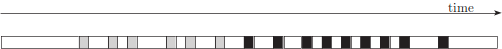
\includegraphics{figures/conc_1a}
    \caption{Αυξητική συλλογή σε σύστημα με μονοπύρηνο επεξεργαστή}
  \end{subfigure}

\begin{subfigure}[b]{1.0\textwidth}
  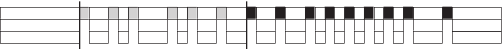
\includegraphics{figures/conc_1b}
  \caption{Αυξητική συλλογή σε σύστημα με πολυπύρηνο επεξεργαστή}
\end{subfigure}
  
  \begin{subfigure}[b]{1.0\textwidth}
    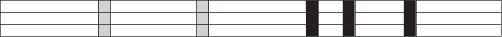
\includegraphics{figures/conc_1c}
    \caption{Παράλληλη αυξητική συλλογή}
  \end{subfigure}
  
  \begin{subfigure}[b]{1.0\textwidth}
    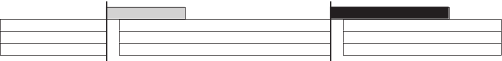
\includegraphics{figures/conc_1d}
    \caption{Σχεδόν-ταυτόχρονη συλλογή}
  \end{subfigure}
  
  \begin{subfigure}[b]{1.0\textwidth}
    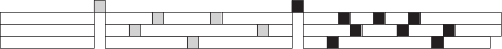
\includegraphics{figures/conc_1e}
    \caption{Σχεδόν-ταυτόχρονη αυξητική συλλογή}
  \end{subfigure}
  
  \begin{subfigure}[b]{1.0\textwidth}
    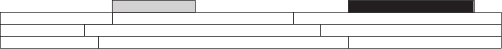
\includegraphics{figures/conc_1f}
    \caption{Εν-τη-πτήσει συλλογή}
  \end{subfigure}
  
  \begin{subfigure}[b]{1.0\textwidth}
    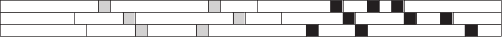
\includegraphics{figures/conc_1g}
    \caption{Εν-τη-πτήσει αυξητική συλλογή}
  \end{subfigure}
    
   \caption[Αυξητική και ταυτόχρονη συλλογή σκουπιδιών]
     {Αυξητική και ταυτόχρονη συλλογή σκουπιδιών. Κάθε μπάρα αναπαριστά μία εκτέλεση σε έναν επεξεργαστή.
      Οι έγχρωμες περιοχές αναπαριστούν διαφορετικούς κύκλους
      συλλογής σκουπιδιών.}
\end{figure}

Υποθέτοντας πώς ο συλλέκτης είναι μονονηματικός και ο
τροποποιητής πολυνηματικός, και πώς ο τροποποιητής
αδρανοποιείται για ένα πολύ σύντομο χρονικό διάστημα στην
αρχή του κύκλου εκτέλεσης του συλλέκτη, ώστε ο τελευταίος να
εξετάσει τις μεταβλητές-ρίζες των πρώτου, τότε έχουμε να
κάνουμε με \textbf{σχεδόν-ταυτόχρονη συλλογή σκουπιδιών}. Εάν
πάλι ο μονονηματικός συλλέκτης εκτελεστεί αυξητικά, όπως πριν,
έχουμε \textbf{σχεδόν-ταυτόχρονη αυξητική συλλογή σκουπιδιών}.
Αξίζει να προσέξουμε πώς στην τελευταία περίπτωση ο
μονονηματικός συλλέκτης μπορεί να εκτελείται σε διαφορετικό 
επεξεργαστή κάθε φορά.

Τέλος, αν θέλουμε να καταργήσουμε τελείως το χρόνο παύσης του
τροποποιητή και επιτρέψουμε στο μονονηματικό συλλέκτη να
εκτελεστεί πραγματικά ταυτόχρονα με αυτόν, τότε ανάλογα με το
αν αυτός εκτελείται συνεχόμενα ή αυξητικά, έχουμε
\textbf{εν-τη-πτήσει συλλογή σκουπιδιών} είτε
\textbf{εν-τη-πτήσει αυξητική συλλογή σκουπιδιών}. Δίνουμε
ιδιαίτερη έμφαση στην ορολογία καθώς μέχρι πρόσφατα οι όροι
παράλληλη, ταυτόχρονη, εν-τη-πτήσει και πραγματικού χρόνου
χρησιμοποιούνταν αυθαίρετα στη βιβλιογραφία.

\section{Ορθότητα ταυτόχρονης συλλογής}
Ένας ορθός ταυτόχρονος συλλέκτης πρέπει να έχει τις ακόλουθες
δύο ιδιότητες:

\begin{itemize}
\item η \textbf{ασφάλεια} απαιτεί τη διατήρηση τουλάχιστον
      όλων των ζωντανών αντικειμένων και
\item η \textbf{ζωντάνια} απαιτεί τον τερματισμό του κύκλου
      συλλογής.
\end{itemize}

\subsection{Η τριχρωματική αφαίρεση}
Η ορθότητα ταυτόχρονων συλλεκτών συνήθως αποδεικνύεται μέσω
αναλλοίωτων που βασίζονται στην τριχρωματική αφαίρεση και
πρέπει να διατηρούνται τόσο από το συλλέκτη όσο και από τον
τροποποιητή. Υπενθυμίζουμε πώς:

\begin{description}
  \item[Λευκά] αντικείμενα είναι εκείνα τα οποία δεν έχουν
    ακόμη ανακαλυφθεί από το συλλέκτη από την αρχή του
    τρέχοντος κύκλου συλλογής. Τα αντικείμενα που παραμένουν
    λευκά στο τέλος του κύκλου θεωρούνται μη-προσβάσιμα
    σκουπίδια.
  \item[Γκρι] αντικείμενα είναι εκείνα τα οποία έχουν ανακαλυφθεί
     από το συλλέκτη, αλλά ένα ή περισσότερα πεδία τους δεν
     έχουν εξετασθεί ακόμα (μπορεί να αναφέρονται σε λευκά
     αντικείμενα).
  \item[Μαύρα] αντικείμενα είναι εκείνα τα οποία έχουν ανακαλυφθεί
     από το συλλέκτη και των οποίων όλα τα πεδία έχουν εξετασθεί
     (και δεν περιέχουν δείκτες προς λευκά αντικείμενα). Τα
     μαύρα αντικείμενα δεν επανεξετάζονται εκτός και αν αλλάξει
     το χρώμα τους.
\end{description}

Ο συλλέκτης σκουπιδιών θεωρείται πώς μετακινεί ένα γκρι μέτωπο
κύματος, που είναι το σύνορο μεταξύ των μαύρων και των λευκών
αντικειμένων. Το πρόβλημα με την ταυτόχρονη εκτέλεση τροποποιητή
και συλλέκτη είναι πώς οι τελευταίοι ενδέχεται να μην μοιράζονται
μια συνεπή εικόνα του σωρού, καθώς το γκρι μέτωπο κύματος δεν
είναι πλέον αυστηρό σύνορο μεταξύ μαύρων και λευκών αντικειμένων.

Αν ο τροποποιητής εκτελείται ταυτόχρονα με το συλλέκτη και
τροποποιήσει πεδία αντικειμένων που βρίσκονται μπροστά από το
μέτωπο κύματος - γκρι αντικείμενα (των οποίων τα πεδία θα πρέπει
να σαρωθούν) ή λευκά αντικείμενα (τα οποία δεν έχουν ανακαλυφθεί 
ακόμη)-τότε δεν υπάρχει πρόβλημα καθώς ο συλλέκτης θα επανεξετάσει
τα αντικείμενα αυτά στο μέλλον (αν είναι ακόμη προσβάσιμα). 
Επίσης δεν υπάρχει πρόβλημα αν τροποποιεί αντικείμενα πίσω από
το μέτωπο κύματος-μαύρα αντικείμενα (των οποίων τα πεδία έχουν
ήδη σαρωθεί)-αρκεί να εισάγονται η διαγράφονται δείκτες μόνο
προς μαύρα ή γκρι αντικείμενα (για τα οποία ο συλλέκτης έχει
ήδη αποφανθεί πώς είναι προσβάσιμα). Όλες οι υπόλοιπες ενημερώσεις
δεικτών μπορεί να οδηγήσουν σε μία κατάσταση όπου τροποποιητής
και συλλέκτης έχουν διαφορετική εικόνα του σωρού.

Αυτό που σε κάθε περίπτωση πρέπει να αποφευχθεί είναι η εισαγωγή
ενός δείκτη προς κάποιο λευκό αντικείμενο στο πεδίο κάποιου μαύρου 
αντικειμένου, καθώς στην περίπτωση αυτή το πρώτο αντικείμενο, παρότι
προσβάσιμο, θα χαθεί (και έτσι θα συλλεχθεί εσφαλμένα).

Ο Wilson \cite{DBLP:conf/iwmm/Wilson92} αποδεικνύει πώς αντικείμενα
χάνονται αν κάποια στιγμή κατά την εξιχνίαση του γράφου αντικειμένων
ισχύουν ταυτόχρονα οι ακόλουθες δύο συνθήκες:

\begin{description}
  \item[Συνθήκη 1:] ο τροποποιητής αποθηκεύει σε ένα μαύρο αντικείμενο
                    ένα δείκτη προς ένα λευκό αντικείμενο και
  \item[Συνθήκη 2:] όλα τα μονοπάτια δια μέσου γκρι αντικειμένων προς
                    το λευκό αντικείμενο καταστρέφονται.
\end{description}

\subsection{Η ασθενής και η ισχυρή τριχρωματική αφαίρεση}
Για να αποφευχθεί η εσφαλμένη συλλογή ζωντανών αντικειμένων,
πρέπει να εξασφαλισθεί πώς οι δύο συνθήκες δεν μπορούν να
επικρατήσουν ταυτόχρονα. Για να μπορεί να εγγυηθεί ο συλλέκτης
πώς δε χάνει προσβάσιμα αντικείμενα, πρέπει να βεβαιωθεί πώς
βρίσκει όλα τα λευκά αντικείμενα προς τα οποία υπάρχει δείκτης
σε μαύρα αντικείμενα. Είναι αρκετό για ένα λευκό αντικείμενο
να είναι προσβάσιμο από κάποιο γκρι αντικείμενο είτε άμεσα
είτε έμμεσα μέσω μιας αλυσίδας λευκών αντικειμένων. Σε αυτήν
την περίπτωση η δεύτερη συνθήκη δεν επικρατεί ποτέ. Η ασθενής
τριχρωματική αναλλοίωτη που πρέπει να διατηρεί ο συλλέκτης
διατυπώνεται ως εξής:

\begin{description}
  \item[Η ασθενής τριχρωματική συνθήκη:] Όλα τα λευκά αντικείμενα
        προς τα οποία υπάρχει δείκτης σε κάποιο μαύρο αντικείμενο
        είναι προσβάσιμα από κάποιο γκρι αντικείμενο, είτε άμεσα,
        είτε μέσω μιας αλυσίδας λευκών αντικειμένων.
\end{description}

Οι ταυτόχρονοι συλλέκτες χωρίς αντιγραφή έχουν το πλεονέκτημα
πώς όλοι οι λευκοί δείκτες αυτόματα μετατρέπονται σε γκρι/μαύρους
όταν το αντικείμενο προς το οποίο δείχνουν σκιάζεται γκρι ή
μαύρο αντίστοιχα. Επομένως η παρουσία λευκών δεικτών στο εσωτερικό
μαύρων αντικειμένων δεν αποτελεί πρόβλημα, καθώς τα αντικείμενα
προς τα οποία δείχνουν, εφόσον τηρείται η ασθενής τριχρωματική
αναλλοίωτη θα σκιαστούν τελικώς γκρι ή μαύρα πριν το τέλος του
τρέχοντος κύκλου συλλογής.

Αντίθετα, οι ταυτόχρονοι συλλέκτες με αντιγραφή είναι πιο
περιορισμένοι καθώς διαθέτουν ρητά δύο αντίγραφα για κάθε
ζωντανό αντικείμενο στο τέλος κάθε κύκλου συλλογής (ένα
λευκό αντίγραφο στο χώρο-από και ένα μαύρο αντίγραφο στο
χώρο-προς), όπου τα λευκά αντικείμενα απορρίπτονται μαζί
με τα αντικείμενα σκουπίδια. Εξ 'ορισμού, ο συλλέκτης δεν
επισκέπτεται ξανά μαύρα αντικείμενα. Επομένως ένας ταυτόχρονος
συλλέκτης με αντιγραφή δεν πρέπει ποτέ να επιτρέψει ένα
πεδίο δείκτης ενός μαύρου αντικειμένου του χώρου-προς να
αναφέρεται προς ένα λευκό αντικείμενο του χώρου-από.
Η ισχυρή τριχρωματική αναλλοίωτη που πρέπει να διατηρεί
ένας τέτοιος συλλέκτης διατυπώνεται ως εξής:

\begin{description}
  \item[Η ισχυρή τριχρωματική συνθήκη:] Δεν υπάρχουν δείκτες
από μαύρα αντικείμενα προς λευκά αντικείμενα.
\end{description}

\subsection{Χρώμα τροποποιητή}
Κατά την κατηγοριοποίηση των αλγορίθμων ταυτόχρονης συλλογής
σκουπιδιών συχνά χρειάζεται να αναφερθούμε στο χρώμα των
αντικειμένων ριζών του τροποποιητή αντιμετωπίζοντας τον
τροποποιητή σαν αντικείμενο. Ένας τροποποιητής είναι γκρι
είτε αν δεν έχει πραγματοποιηθεί ακόμη εξιχνίαση από τις
ρίζες του είτε αν οι ρίζες του έχουν σαρωθεί και πρέπει
να σαρωθούν εκ νέου. Αυτό σημαίνει πώς οι ρίζες ενός γκρι
τροποποιητή μπορούν να αναφέρονται σε αντικείμενα όλων των
χρωμάτων. Ένας τροποποιητής είναι μαύρος αν έχει πραγματοποιηθεί
η εξιχνίαση από τις ρίζες του και αυτές δε θα σαρωθούν ξανά.
Υπό την ισχυρή τριχρωματική αναλλοίωτη αυτό σημαίνει πώς
οι ρίζες ενός μαύρου τροποποιητή μπορούν να αναφέρονται
μόνο σε μαύρα ή γκρι αντικείμενα. Υπό την ασθενή τριχρωματική
αναλλοίωτη, οι ρίζες ενός μαύρου τροποποιητή μπορούν να
αναφέρονται σε λευκά αντικείμενα, αρκεί τα τελευταία να είναι
προσβάσιμα από κάποιο γκρι αντικείμενο είτε έμμεσα είτε μέσω
μιας αλυσίδας λευκών αντικειμένων.

Το χρώμα του τροποποιητή έχει επιπτώσεις στον τερματισμό
ενός κύκλου συλλογής. Εξ 'ορισμού, αλγόριθμοι ταυτόχρονης
συλλογής σκουπιδιών πρέπει να σαρώσουν ξανά τις ρίζες ενός
γκρι τροποποιητή. Αυτό ενδέχεται να οδηγήσει σε καινούρια
εργασία εξιχνίασης αν βρεθεί ένας όχι μαύρος δείκτης. Όταν
η εξιχνίαση αυτή ολοκληρωθεί, οι ρίζες πρέπει να σαρωθούν
ξανά καθώς ο τροποποιητής μπορεί και πάλι στο ενδιάμεσο
να έχει αποθηκεύσει ένα μη μαύρο δείκτη κ.ό.κ. Στη χειρότερη
περίπτωση μπορεί να χρειαστεί να ανασταλεί η εκτέλεση όλων
των νημάτων τροποποιητών ώστε να σαρωθούν για μια τελευταία
φορά οι ρίζες τους.

Οι εν-τη-πτήσει συλλέκτες ξεχωρίζουν τα νήματα τροποποιητές
καθώς δεν αναστέλλουν την εκτέλεση όλων ταυτόχρονα για να
εξετάσουν τις ρίζες τους. Οι συλλέκτες αυτής της κατηγορίας
πρέπει να λειτουργήσουν με νήματα τροποποιητές διαφορετικών
χρωμάτων.

\subsection{Χρώμα εκχώρησης}
Το χρώμα του τροποποιητή επηρεάζει επίσης το χρώμα που
λαμβάνει ένα αντικείμενο κατά την εκχώρησή του, καθώς ο
ο δείκτης προς αυτό αποθηκεύεται στον τροποποιητή, ο οποίος
ανάλογα με το χρώμα του πρέπει να διατηρεί την ασθενή ή
ισχυρή τριχρωματική αναλλοίωτη. Το χρώμα εκχώρησης επηρεάζει
επίσης το πόσο γρήγορα θα απελευθερωθεί ένα αντικείμενο από
τη στιγμή που αυτό καθίσταται μη προσβάσιμο. Εάν ένα αντικείμενο
εκχωρείται ως μαύρο ή γκρι τότε δε θα ελευθερωθεί στη διάρκεια
του τρέχοντος κύκλου συλλογής (διότι τα μαύρα και γκρι αντικείμενα
θεωρούνται ζωντανά) ακόμη και εάν καταστεί μη προσβάσιμο.
Σε ένα γκρι τροποποιητή τα αντικείμενα μπορούν να εκχωρούνται
ως λευκά και έτσι να αποφεύγεται η χωρίς λόγο διατήρηση
νέων αντικειμένων. Αντίθετα, σε ένα μαύρο τροποποιητή νέα
αντικείμενα δεν μπορούν να εκχωρούνται ως λευκά εκτός και
αν διατηρείται η ασθενής τριχρωματική αναλλοίωτη και υπάρχει
κάποια εγγύηση πώς ο λευκός δείκτης θα αποθηκευθεί σε
ένα ζωντανό αντικείμενο που βρίσκεται μπροστά από το μέτωπο
κύματος και δε θα συλλεγεί εσφαλμένα. Τέλος, ένα καινούριο
αντικείμενο δεν περιέχει (ακόμη) δείκτες και συνεπώς
είναι πάντα ασφαλές να εκχωρείται ως μαύρο.

\section{Τεχνικές φράγματος για ταυτόχρονη συλλογή}
Σύμφωνα με τον Pirinen, \cite{DBLP:conf/iwmm/Pirinen98} οι
τεχνικές φράγματος που διατηρούν μία εκ των δύο τριχρωματικών
αναλλοίωτων βασίζονται σε έναν αριθμό από ενέργειες για να
διαχειρισθούν την εισαγωγή και διαγραφή δεικτών. Οι τεχνικές
αυτές μπορούν:
\begin{itemize}
\item Να αυξήσουν το μέγεθος του μετώπου κύματος, \textbf{σκιάζοντας}
  γκρι ένα αντικείμενο αν αυτό ήταν λευκό. Η σκίαση ενός γκρι
  ή μαύρου αντικειμένου δεν έχει κανένα αποτέλεσμα.
\item Να μετακινήσουν προς τα εμπρός το μέτωπο κύματος \textbf{σαρώνοντας}
  ένα αντικείμενο για να το χρωματίσουν μαύρο.
\item Να μετακινήσουν προς τα πίσω το μέτωπο κύματος \textbf{αντιστρέφοντας}
  το χρώμα ενός αντικειμένου από μαύρο σε γκρι.
\end{itemize}

\subsection{Τεχνικές γκρι τροποποιητή}
Αρχικά παρουσιάζουμε προσεγγίσεις που λειτουργούν με γκρι τροποποιητή.
Όλες αυτές οι τεχνικές διατηρούν την ισχυρή αναλλοίωτη χρησιμοποιώντας
ένα \textbf{φράγμα εισαγωγής} κατά την εγγραφή αναφορών στο σωρό για
να αποτρέψουν την αποθήκευση λευκών δεικτών σε μαύρα αντικείμενα.
Καθώς ο τροποποιητής είναι γκρι, δεν απαιτείται φράγμα εγγραφής.

\begin{itemize}
  \item Το φράγμα εγγραφής του Steele, \cite{DBLP:journals/cacm/Steele75} το
    οποίο φαίνεται στον αλγόριθμο~\ref{alg:conc_1} παρουσιάζει
    τη μεγαλύτερη ακρίβεια ανάμεσα σε όλες τις τεχνικές απλώς επειδή
    σημειώνει το αντικείμενο προέλευσης υπό τροποποίηση. Δε μεταβάλλει
    καμία απόφαση όσον αφορά την προσβασιμότητα ενός αντικειμένου, αλλά
    προκαλεί την μετακίνηση του μετώπου κύματος προς τα πίσω αλλάζοντας
    το χρώμα του τροποποιημένου μαύρου αντικειμένου από μαύρο σε γκρι.
    Αναβάλλει την απόφαση σχετικά με την προσβασιμότητα του λευκού
    αντικειμένου προορισμού μέχρις ότου το μαύρο αντικείμενο προέλευσης
    σαρωθεί εκ νέου (ο εισαχθείς δείκτης ενδέχεται να έχει διαγραφεί
    στο ενδιάμεσο). Η ακρίβεια αυτή έρχεται εις βάρος της προόδου,
    καθώς το μέτωπο κύματος μετακινείται προς τα πίσω.

   \item Ο Boehm κ.ά. \cite{DBLP:conf/pldi/BoehmDS91} υλοποίησαν μια
   παραλλαγή του φράγματος εγγραφής του Steele η οποία αγνοεί το χρώμα του
   εισαγόμενου δείκτη, όπως φαίνεται στον αλγόριθμο~\ref{alg:conc_1}.
   Αρχικά υλοποίησαν αυτό το φράγμα χρησιμοποιώντας
   τα βρώμικα bits της εικονικής μνήμης για να καταγράφουν τις
   τροποποιημένες σελίδες χωρίς να χρειάζεται έτσι οι λειτουργίες
   εγγραφής πεδίων αντικειμένων του σωρού να παρακολουθούνται σε επίπεδο
   λογισμικού. Η αρχική υλοποίηση του φράγματος μάλιστα δεν ήλεγχε
   πώς το αντικείμενο προέλευσης είναι μαύρο, καθιστώντας το φράγμα
   λιγότερο ακριβές. Ο τερματισμός της συλλογής γινόταν με παύση
   του κόσμου οπότε και οι βρώμικες σελίδες σαρώνονταν εκ νέου.

  \item Ο Dijkstra κ.ά. \cite{DBLP:conf/ac/DijkstraLMSS75,
   DBLP:journals/cacm/DijkstraLMSS78} σχεδίασαν ένα φράγμα εγγραφής
   (αλγόριθμος~\ref{alg:conc_1} λιγότερο
   ακριβές από το αντίστοιχο του Steele: το αντικείμενο προορισμού
   του εισαγόμενου δείκτη σκιάζεται ως προσβάσιμο (μη λευκό) παρότι
   ο δείκτης μπορεί στη συνέχεια να διαγραφεί. Αυτή η απώλεια
   ακρίβειας συμβάλλει στην πρόοδο καθώς το μέτωπο κύματος
   μετακινείται προς τα εμπρός. Η αρχική μάλιστα υλοποίηση του
   φράγματος ήταν ακόμη λιγότερο ακριβής καθώς το αντικείμενο
   προορισμού του εισαγόμενου δείκτη σκιαζόταν χωρίς να ελέγχεται
   πώς το χρώμα του αντικειμένου προέλευσης είναι μαύρο. Η παράλειψη
   αυτού του ελέγχου επιτρέπει τη χαλάρωση της απαίτησης για ατομική
   εκτέλεση όλου του φράγματος εγγραφής, υπό την προϋπόθεση βέβαια
   πώς οι ξεχωριστές λειτουργίες της αποθήκευσης και της σκίασης
   εκτελούνται ατομικά.
\end{itemize}

\subsection{Τεχνικές μαύρου τροποποιητή}
Οι πρώτες δύο προσεγγίσεις εφαρμόζουν αυξητική ενημέρωση για
τη διατήρηση της ισχυρής αναλλοίωτης χρησιμοποιώντας ένα φράγμα
ανάγνωσης για να αποτρέψουν τον τροποποιητή από την απόκτηση
λευκών δεικτών (δηλαδή να αποτρέψουν την εισαγωγή ενός λευκού
δείκτη σε ένα μαύρο τροποποιητή). Η τρίτη προσέγγιση χρησιμοποιεί
ένα \textbf{φράγμα διαγραφής} στις λειτουργίες εγγραφής δεικτών
στο σωρό για τη διατήρηση της ασθενούς αναλλοίωτης. Υπό την
ασθενή τριχρωματική αναλλοίωτη ένας μαύρος τροποποιητής μπορεί
να διατηρεί λευκούς δείκτες: είναι μαύρος καθώς δεν απαιτείται
η εκ νέου σάρωση των ριζών του και έτσι μπορεί να φορτώνει
τιμές δεικτών προς λευκά αντικείμενα, αφού το φράγμα εγγραφής
προστατεύει τα τελευταία από μια πιθανή διαγραφή.

\begin{itemize}
  \item Ο Baker \cite{DBLP:journals/cacm/Baker78} χρησιμοποίησε
    το φράγμα ανάγνωσης που φαίνεται στον αλγόριθμο~\ref{alg:conc_2}. Η
    προσέγγισή του είναι λιγότερο ακριβής από την προσέγγιση του
    Dijkstra κ.ά. καθώς εσφαλμένα διατηρεί αντικείμενα (που θα
    ήταν λευκά) απλώς επειδή κάποιο νήμα τροποποιητής φορτώνει
    τις τιμές δεικτών προς αυτά κατά τη διάρκεια ενός κύκλου
    συλλογής (σε αντίθεση με λευκά αντικείμενα που εισάγονται
    πίσω από το μέτωπο κύματος και τα οποία πρέπει να διατηρηθούν).
    Το φράγμα ανάγνωσης του Baker σχεδιάσθηκε αρχικώς για ένα
    συλλέκτη αντιγραφής, όπου η ενέργεια της σκίασης αντιγράφει
    ένα αντικείμενο από το χώρο-από στο χώρο-προς και έτσι η
    ρουτίνα \textproc{shade} επιστρέφει τη διεύθυνση του αντιγράφου
    του αντικειμένου στο χώρο-προς. 
  \item Ο Appel κ.ά. \cite{DBLP:conf/pldi/AppelEL88} υλοποίησαν
    μία λιγότερο ακριβή παραλλαγή του φράγματος ανάγνωσης του
    Baker, (αλγόριθμος~\ref{alg:conc_2} χρησιμοποιώντας μηχανισμούς
    προστασίας σελίδων εικονικής μνήμης για την παγίδευση των
    προσβάσεων νημάτων τροποποιητών σε γκρι σελίδες με αποτέλεσμα
    να μη χρειάζεται η παρακολούθηση των λειτουργιών ανάγνωσης σε
    επίπεδο λογισμικού. Μια παγιδευμένη πρόσβαση μπορεί να
    ολοκληρωθεί μετά τη σάρωση της αντίστοιχης σελίδας (και την
    άρση του αποκλεισμού της). Αυτό το φράγμα ανάγνωσης μπορεί
    επίσης να χρησιμοποιηθεί και από ένα ταυτόχρονο συλλέκτη
    αντιγραφής αφού η σάρωση θα προωθήσει τυχόν πεδία δείκτες
    προς αντικείμενα του χώρου-προς του αντικειμένου προέλευσης.   
  \item Οι Abraham και Patel \cite{DBLP:conf/icpp/AbrahamP87},
    και ο Yuasa \cite{DBLP:journals/jss/Yuasa90} σχεδίασαν
    ανεξάρτητα το φράγμα διαγραφής που φαίνεται στον αλγόριθμο~\ref{alg:conc_2}.
    Αυτό το φράγμα διαγραφής παρουσιάζει τη μικρότερη
    ακρίβεια από όλες τις τεχνικές καθώς διατηρεί κάθε μη
    προσβάσιμο αντικείμενο προς το οποίο ο τελευταίος δείκτης
    διαγράφηκε κατά τη διάρκεια του κύκλου συλλογής. 
\end{itemize}

\begin{algorithm}
  \caption{Φράγματα γκρι τροποποιητή}
  \label{alg:conc_1}
  \subcaption{\centering Φράγμα εγγραφής του Steele}%\label{alg:conc_1a}
  \hrulefill
  \begin{algorithmic}[1]
    \Procedure{Write}{$src$, $i$, $ref$}
      \State \textbf{atomic}
      \State $src[i] \gets ref$
      \If{\Call{isBlack}{$src$}}
        \If{\Call{isWhite}{$ref$}}
          \State \Call{revert}{$src$}
        \EndIf
      \EndIf
    \EndProcedure
  \end{algorithmic}
  \hrulefill
  \subcaption{\centering Φράγμα εγγραφής του Boehm κ.ά}%\label{alg:conc_1b}
  \hrulefill
  \begin{algorithmic}[1]
    \Procedure{Write}{$src$, $i$, $ref$}
      \State \textbf{atomic}
      \State $src[i] \gets ref$
      \If{\Call{isBlack}{$src$}}
        \State \Call{revert}{$src$}
      \EndIf
    \EndProcedure
  \end{algorithmic}
  \hrulefill
  \subcaption{\centering Φράγμα εγγραφής του Dijkstra κ.ά}%\label{conc_1c}
  \hrulefill
  \begin{algorithmic}[1]
    \Procedure{Write}{$src$, $i$, $ref$}
      \State \textbf{atomic}
      \State $src[i] \gets ref$
      \If{\Call{isBlack}{$src$}}
        \State \Call{shade}{$src$}
      \EndIf
    \EndProcedure
  \end{algorithmic}
\end{algorithm}

\begin{algorithm}
  \caption{Φράγματα μαύρου τροποποιητή}
  \label{alg:conc_2}
  \subcaption{\centering Φράγμα ανάγνωσης του Baker}%\label{conc_2a}
  \hrulefill
  \begin{algorithmic}[1]
    \Function{Read}{$src$, $i$}
      \State \textbf{atomic}
      \State $ref \gets src[i]$
      \If{\Call{isGrey}{$src$}}
          \State $ref \gets$ \Call{shade}{$src$}
      \EndIf
      \State \Return{$ref$}
    \EndFunction
  \end{algorithmic}
  \hrulefill
  \subcaption{\centering Φράγμα ανάγνωσης του Appel κ.ά}%\label{conc_2b}
  \hrulefill
  \begin{algorithmic}[1]
    \Function{Read}{$src$, $i$}
      \State \textbf{atomic}
      \State $src[i] \gets ref$
      \If{\Call{isGrey}{$src$}}
        \State \Call{scan}{$src$}
      \EndIf
      \State \Return{$src[i]$}
    \EndFunction
  \end{algorithmic}
  \hrulefill
  \subcaption{\centering Φράγμα εγγραφής των Abraham κ.ά / Yuasa}%\label{conc_2c}
  \hrulefill
  \begin{algorithmic}[1]
    \Procedure{Write}{$src$, $i$, $ref$}
      \State \textbf{atomic}
      \If{\Call{isGrey}{$src$} \textbf{or} \Call{isWhite}{$src$}}
        \State \Call{shade}{$src[i]$}
      \EndIf
      \State $src[i] \gets ref$
    \EndProcedure
  \end{algorithmic}
\end{algorithm}


\section{Ταυτόχρονη σήμανση και εκκαθάριση}
Στην ενότητα αυτή εξετάζουμε την
\textbf{ταυτόχρονη συλλογή με σήμανση και εκκαθάριση}. Όπως
είδαμε και πριν, το πιο σημαντικό θέμα όσον αφορά έναν
ταυτόχρονο συλλέκτη είναι η εξασφάλιση της ορθότητας.
Συλλέκτης και τροποποιητής οφείλουν να συνεργάζονται
προκειμένου να διαβεβαιώσουν πώς μοιράζονται μια συνεπή
εικόνα της μνήμης του σωρού. Ο τροποποιητής από την πλευρά
του οφείλει να αποτρέπει ζωντανά αντικείμενα να μην είναι
ορατά στο συλλέκτη, ενώ ένας συλλέκτης που μετακινεί
αντικείμενα οφείλει να εξασφαλίζει πώς ο συλλέκτης
χρησιμοποιεί τις σωστές διευθύνσεις των μετακινηθέντων
αντικειμένων.

Οι ταυτόχρονοι συλλέκτες με σήμανση και εκκαθάριση είναι οι
απλούστεροι από όλους τους ταυτόχρονους συλλέκτες. Καθώς δε
μεταβάλλουν πεδία δείκτες, ο τροποποιητής μπορεί ελεύθερα
να διαβάζει τις τιμές δεικτών χωρίς να χρειάζεται να
προστατευθεί από το συλλέκτη. Δεν υπάρχει επομένως εγγενής
ανάγκη για φράγμα ανάγνωσης όταν χρησιμοποιείται μη μετακινών
συλλέκτης. Ειδάλλως, η χρήση φράγματος ανάγνωσης για τη
διατήρηση της ισχυρής αναλλοίωτης σε ένα σύστημα με συλλέκτη
που δεν μετακινεί αντικείμενα θεωρείται πολύ ακριβή, καθώς οι
αναγνώσεις δεδομένων του σωρού από τον τροποποιητή είναι πολύ
συχνότερες από ότι οι εγγραφές. Για παράδειγμα, ο Zorn \cite{DBLP:conf/lfp/Zorn90}
μέτρησε και υπολόγισε το ποσοστό των φορτώσεων και αποθηκεύσεων
δεικτών στο σύστημα SPUR LISP από 13\% έως 15\% και 4\%
αντίστοιχα. Η εξαίρεση στον παραπάνω γενικό κανόνα προκύπτει
όταν τεχνικές βελτιστοποιήσεων του μεταγλωττιστή χρησιμοποιούνται
για να εξαλείψουν τα περιττά φράγματα, όπως από το Hosking κ.ά. \cite{DBLP:conf/oopsla/HoskingC99}
και τους Zee και Rinard \cite{DBLP:conf/oopsla/ZeeR02},
ή για να ενσωματώσουν ένα τμήμα του έργου των φραγμάτων στο ήδη
υπάρχον κόστος που αφορά τον έλεγχο των δεικτών έναντι της ειδικής τιμής \textbf{null},
όπως από το Bacon κ.ά. \cite{DBLP:conf/lctrts/BaconCR03}. Γι αυτό το λόγο οι
ταυτόχρονοι συλλέκτες με σήμανση και εκκαθάριση συνήθως 
χρησιμοποιούν το φράγμα αυξητικής ενημέρωσης του Dijkstra 
\cite{DBLP:conf/ac/DijkstraLMSS75,DBLP:journals/cacm/DijkstraLMSS78},
είτε το φράγμα εγγραφής εισαγωγής του Steele  \cite{DBLP:journals/cacm/Steele75},
είτε το φράγμα εγγραφής εισαγωγής του Boehm κ.ά. \cite{DBLP:conf/pldi/BoehmDS91},
είτε το φράγμα εγγραφής διαγραφής του Yuasa \cite{DBLP:journals/jss/Yuasa90}.

\subsection{Αρχικοποίηση}
Αντί να επιτρέπεται η εκτέλεση του τροποποιητή μέχρις ότου η μνήμη να εξαντληθεί, οι ταυτόχρονοι 
συλλέκτες μπορούν να εκτελούνται ακόμη και όταν ο τροποποιητής ακόμα μπορεί να δεσμεύει μνήμη 
προς δημιουργία αντικειμένων. Αν μία συλλογή  ενεργοποιηθεί πολύ αργά, ενδέχεται να μην υπάρχει 
επαρκής μνήμη για την ικανοποίηση ενός αιτήματος εκχώρησης, στην οποία περίπτωση θα καθυστερήσει 
η εκτέλεση του τροποποιητή μέχρις ότου τελειώσει ο κύκλος συλλογής. Τη στιγμή που εκκινεί ο 
κύκλος συλλογής, η ρυθμαπόδοση σταθερής κατάστασης του συλλέκτη πρέπει να επαρκεί για την 
ολοκλήρωση του κύκλου πριν εξαντληθεί η μνήμη από τον τροποποιητή και να επιδρά στη ρυθμαπόδοση 
του τελευταίου το ελάχιστο δυνατό. Το πότε και πώς θα ενεργοποιηθεί ένας κύκλος συλλογής 
εξασφαλίζοντας τη διαθεσιμότητα επαρκούς μνήμης για την ικανοποίηση των αιτημάτων του τροποποιητή 
και ενώ εκτελείται ο συλλέκτης, καθώς και το πότε ο κύκλος θα τελειώσει ούτως ώστε η μνήμη από
τα σκουπίδια να ανακτηθεί εξαρτώνται από τη δρομολόγηση εργασιών συλλογής παράλληλα με την 
εκτέλεση του τροποποιητή.

Ο αλγόριθμος~\ref{alg:conc_3} απεικονίζει την αλληλουχία ενεργειών κατά την εκχώρηση μνήμης στον 
τροποποιητή για έναν ταυτόχρονο συλλέκτη με σήμανση και εκκαθάριση ο οποίος δρομολογεί ένα 
ποσό έργου συλλογής αυξητικά σε κάθε εκχώρηση μνήμης μέσω της διαδικασίας \textenglish{\textproc{collectEnough}}. 
Η συνάρτηση \textenglish{\textproc{behind}} αποφασίζει σχετικά με το πότε και πόσο έργο συλλογής πρέπει να 
εκτελεστεί, εξασφαλίζοντας πώς ο τροποποιητής δεν βρίσκεται πολύ μπροστά από το συλλέκτη ώστε η 
συνάρτηση \textenglish{\textproc{allocate}} να μην μπορεί να ικανοποιήσει αιτήματα μνήμης.

Ο αλγόριθμος~\ref{alg:conc_4} δείχνει τι ακριβώς συμβαίνει όταν δρομολογείται η εκτέλεση έργου 
συλλογής. Η αρχικά κενή λίστα εργασιών γεμίζει με αναφορές προς αντικείμενα προς τα οποία δείχνουν 
οι ρίζες. Υποθέτοντας πώς η εξέταση των ριζών σημαίνει την αναστολή λειτουργίας και εξέταση όλων 
των νημάτων τροποποιητών, σε αυτό το σημείο κάνενα νήμα τροποποιητής δεν περιλαμβάνει κάποια 
λευκή αναφορά. Επομένως έχουμε έναν σχεδόν ταυτόχρονο τρόπο λειτουργίας, με μία μικρή φάση παύσης 
για την αρχικοποίηση της συλλογής. Τα γκρι πλέον αντικείμενα ρίζες αναπαριστούν το αρχικό μέτωπο 
κύματος από το οποίο θα συνεχίσει η εξερεύνηση του γράφου των αντικειμένων. Εφόσον οι ρίζες τους
έχουν εξετασθεί, τα νήματα τροποποιητές μπορούν πλέον να συνεχίσουν είτε ως μαύρα (εφόσον δεν 
έχουν λευκές αναφορές) είτε ως γκρι, ανάλογα με τα φράγματα τροποποίησης που είναι σε χρήση.

\begin{algorithm}
  \caption{Σχεδόν-ταυτόχρονη σήμανση και εκκαθάριση: εκχώρηση}
  \label{alg:conc_3}
  \begin{algorithmic}[1]
    \Function{New}{\null}
      \State \Call{collectEnough}{\null}
      \State $ref \gets$ \Call{allocate}{\null} \Comment{must initialize black if collector is black}
      \If{$ref = \textbf{null}$}
        \State error ''Out of memory''
      \EndIf
      \State \Return{$ref$}
    \EndFunction
    \Statex
    \Function{collectEnough}{\null}
      \State \textbf{atomic}
      \While{\Call{behind}{\null}}
        \If{\textbf{not} \Call{markSome}{\null}}
          \State \Return{null}
        \EndIf
      \EndWhile
    \EndFunction
  \end{algorithmic}
\end{algorithm}

Η αναστολή της λειτουργίας των νημάτων τροποποιητών ενδέχεται να οδηγήσει σε απαράδεκτες
παύσεις. Η χρήση γκρι φραγμάτων τροποποίησης καθιστά εφικτή την ενεργοποίηση των φραγμάτων και την 
αναβολή της εξέτασης όλων των ριζών, η οποία πραγματοποιείται αργότερα και ενώ ταυτόχρονα εκτελούνται 
τα νήματα τροποποιητές. 

\subsection{Τερματισμός σήμανσης}
Ο τερματισμός της φάσης σήμανσης για ένα μαύρο τροποποιητή είναι μία σχετικά απλή διαδικασία και 
συμβαίνει όταν δεν υπάρχουν πλέον γκρι αντικείμενα στη λίστα εργασιών. Σε αυτό το σημείο, θεωρώντας 
ακόμη και την ασθενή τριχρωματική αναλλοίωτη ο τροποποιητής μπορεί να περιλαμβάνει μόνο μαύρες 
αναφορές, καθώς δεν υπάρχουν λευκά αντικείμενα προσβάσιμα από γκρι αντικείμενα (δεν υπάρχουν καθόλου 
γκρι αντικείμενα). Καθώς ο τροποποιητής είναι μαύρος, δεν απαιτείται η επανεξέταση των ριζών του.

Ο τερματισμός της φάσης σήμανσης για έναν γκρι τροποποιητή είναι λίγο πιο περίπλοκος, καθώς ο 
τροποποιητής μπορεί να έχει αποκτήσει λευκούς δείκτες από τη στιγμή που εξετάστηκαν οι ρίζες του για 
την αρχικοποίηση της συλλογής. Επομένως οι ρίζες ενός γκρι τροποποιητή πρέπει να επανεξετασθούν πριν 
η φάση σήμανσης τερματιστεί. Εάν η επανεξέταση δεν ανακαλύψει φρέσκα γκρι αντικείμενα, τότε η φάση 
της σήμανσης τερματίζεται και εκκινεί η φάση της εκκαθάρισης. Η τελευταία μπορεί να είναι πρόθυμη ή 
οκνηρή. 

\begin{algorithm}
  \caption{Σχεδόν-ταυτόχρονη σήμανση}
  \label{alg:conc_4}
  \begin{algorithmic}[1]
    \State \textbf{shared} $worklist \gets empty$
    \Statex
    \Function{markSome}{\null}
      \If{\Call{isEmpty}{$worklist$}} \Comment{initiate collection}
        \State \Call{scan}{$Roots$} \Comment{invariant: collector holds no white references}
        \If{\Call{isEmpty}{$worklist$}} \Comment{invariant: no more grey references}
          \State /* marking terminates */
          \State \Call{sweep}{\null} \Comment{lazy or eager sweep}
          \State \Return{\textbf{false}} \Comment{terminate marking}
        \EndIf
      \EndIf
      \State /* collection continues */
      \State $ref \gets$ \Call{remove}{$worklist$}
      \State \Call{scan}{$ref$} \Comment{continue marking, if still behind}
      \State \Return{\textbf{true}}
    \EndFunction
    \Statex
    \Procedure{shade}{$ref$}
      \If{\textbf{not} \Call{isMarked}{\null}}
        \State \Call{setMarked}{$ref$}
        \State \Call{add}{$worklist$, $ref$}
      \EndIf
    \EndProcedure
    \Statex
    \Procedure{scan}{$ref$}
      \ForAll{$fld \; \textbf{in} \; Pointers(ref)$}
        \State $child \gets *fld$
        \If{$child \neq \textbf{null}$}
          \State \Call{shade}{$child$}
        \EndIf
      \EndFor
    \EndProcedure
    \Statex
    \Function{revert}{$ref$}
      \State \Call{add}{$worklist$, $ref$}
    \EndFunction
    \Statex
    \Function{isWhite}{$ref$}
      \State \Return{\textbf{not} \Call{isMarked}{$ref$}}
    \EndFunction
    \Statex
    \Function{isGrey}{$ref$}
      \State \Return{$ref \textbf{in} worklist$}
    \EndFunction
    \Statex
    \Function{isBlack}{$ref$}
      \State \Return{\Call{isMarked}{$ref$} \textbf{and} \textbf{not} \Call{isGrey}{$ref$}}
    \EndFunction
  \end{algorithmic}
\end{algorithm}

\subsection{Ταυτόχρονη σήμανση και ταυτόχρονη εκκαθάριση}
Μέχρι στιγμής έχουμε θεωρήσει την εκτέλεση μόνο της φάσης
της σήμανσης ταυτόχρονα με τον τροποποιητή και πως η φάση
της εκκαθάρισης έπεται αυτής σειριακά. Εάν η εκκαθάριση
είναι οκνηρή, αιτήματα εκχώρησης μνήμης από τον τροποποιητή
ενδέχεται να ενεργοποιούν την ταυτόχρονη εκκαθάριση που
αντιστοιχεί στη σήμανση του προηγούμενου κύκλου συλλογής
και ενώ ήδη ένας νέος κύκλος συλλογής βρίσκεται στην επόμενη
φάση σήμανσης. Το γεγονός αυτό μπορεί να προκαλέσει σύγχυση
όσον αφορά τα χρώματα των αντικειμένων. Θα πρέπει με κάποιο
τρόπο να μπορούν να διαχωρισθούν τα πραγματικά λευκά
σκουπίδια από την προηγούμενη φάση σήμανσης (τα οποία πρέπει
να εκκαθαρισθούν) από τα μέχρι μη σημασμένα λευκά αντικείμενα
της τρέχουσας φάσης σήμανσης. Ο Lamport \cite{lamport1976garbage}
ξεχωρίζει μεταξύ των δύο ειδών αντικειμένων χρησιμοποιώντας
ένα καινούριο χρώμα, το μωβ. Όταν ολοκληρώνεται η φάση σήμανσης,
όλα τα λευκά αντικείμενα σκουπίδια χρωματίζονται μωβ. Η
εκκαθάριση θα συλλέξει τα μωβ αντικείμενα, προσθέτοντας
τα στην ελεύθερη λίστα και επαναχρωματίζοντας σε μαύρα
ή λευκά, ανάλογα με το χρώμα του εκχωρητή.

Ο Lamport χρησιμοποιεί πολλαπλά ταυτόχρονα νήματα σήμανσης και νήματα
εκκαθάρισης και ορίζει έναν κύκλο συλλογής ως εξής:

\begin{enumerate}
  \item Περίμενε μέχρις ότου όλα τα νήματα σήμανσης και όλα τα νήματα
        εκκαθάρισης ολοκληρώσουν τις εργασίες τους.
  \item Άλλαξε το χρώμα των λευκών αντικειμένων σε μωβ και των μαύρων
        αντικειμένων σε λευκό (για την αποφυγή αιωρούμενων σκουπιδιών)
        ή γκρι (στην περίπτωση που το αντικείμενο έχει σκιασθεί ταυτόχρονα
        από το φράγμα εγγραφής ενός νήματος τροποποιητή).
  \item Σκίασε όλες τις ρίζες.
  \item Εκκίνησε όλα τα νήματα σήμανσης και όλα τα νήματα εκκαθάρισης.
\end{enumerate}

Η σήμανση αγνοεί όλα τα μωβ αντικείμενα: ένα νήμα τροποποιητής δεν μπορεί
ποτέ να αποκτήσει μια αναφορά προς ένα μωβ αντικείμενο και συνεπώς τα
γκρι αντικείμενα δε δείχνουν ποτέ σε μωβ αντικείμενα και τα μωβ αντικείμενα
δε σκιάζονται ποτέ. Το πρόβλημα με αυτή την προσέγγιση είναι πώς 
για να εκκινήσει η εκκαθάριση πρέπει να έχει αλλαχθεί το χρώμα από
λευκό σε μωβ όλων των αντικειμένων σκουπιδιών του προηγούμενου κύκλου.
Παρόμοια, κατά την έναρξη της σήμανσης, πρέπει το χρώμα όλων των
μαύρων αντικειμένων του προηγούμενου κύκλου να αλλαχθεί σε λευκό
ή γκρι.

\subsection{Εν-τη-πτήσει σήμανση}
Μέχρι στιγμής έχουμε υποθέσει πώς, είτε πρόκειται για την
εκκίνηση είτε για τον τερματισμό της φάσης σήμανσης, αναστέλλεται
η εκτέλεση όλων των νημάτων τροποποιητών ταυτόχρονα για να
σαρωθούν οι ρίζες τους. Στη συνέχεια, κάθε νήμα τροποποιητής
συνεχίζει να εκτελείται είτε ως μαύρο ή γκρι ανάλογα με το φράγμα
εγγραφής που χρησιμοποιεί. Αυτές οι παύσεις του κόσμου μειώνουν
τον ταυτοχρονισμό. Μια εναλλακτική προσέγγιση είναι οι ρίζες
κάθε νήματος τροποποιητή να σαρώνονται ξεχωριστά και ταυτόχρονα
με την εκτέλεση των υπόλοιπων νημάτων τροποποιητών. Η διαφορετική
ταυτόχρονη εκτέλεση ορισμένων νημάτων τροποποιητών ως γκρι και
ορισμένων άλλων ως μαύρων εισάγει επιπλέον πολυπλοκότητα και
επηρεάζει επίσης τον εντοπισμό του τερματισμού της φάσης σήμανσης.

Η εν-τη-πτήσει συλλογή ποτέ δεν αναστέλλει την εκτέλεση όλων
των νημάτων τροποποιητών ταυτόχρονα, αλλά εμπλέκει κάθε ένα από
αυτά σε μία σειρά \textbf{χειραψιών} που δεν απαιτούν καθολικό
συγχρονισμό. Ο συλλέκτης παρακινεί ασύγχρονα όλα τα νήματα
τροποποιητές, ένα προς ένα, να σταματήσουν την εκτέλεσή τους σε
κάποιο βολικό χρονικό σημείο. Ο συλλέκτης μπορεί στη συνέχεια
να εξετάσει (και πιθανώς τροποποιήσει) τις ρίζες κάθε νήματος
τροποποιητή πριν του επιτρέψει τη συνέχιση της εκτέλεσής του.
Η προσέγγιση αυτή επιτρέπει την ταυτόχρονη εκτέλεση των υπόλοιπων
νημάτων τροποποιητών κατά την παύση της εκτέλεσης ενός νήματος
τροποποιητή.

Η χρήση χειραψιών εισήχθη για πρώτη φορά από τους Doligez και
Leroy \cite{DBLP:conf/popl/DoligezL93} και Doligez και Gonthier
\cite{DBLP:conf/popl/DoligezG94} σε ένα συλλέκτη σήμανσης
και εκκαθάρισης για τη γλώσσα προγραμματισμού ML.

\section{Ταυτόχρονη Αντιγραφή}
Σε αυτήν και την επόμενη ενότητα εξετάζουμε πώς μπορεί να
ελαχιστοποιηθεί ο κατακερματισμός του σωρού αντιγράφοντας
ζωντανά αντικείμενα από το χώρο-από στο χώρο-προς ταυτόχρονα
με την εκτέλεση του τροποποιητή.

Η ορθότητα της συλλογής σκουπιδιών με ταυτόχρονη αντιγραφή
απαιτεί να προστατευθούν τόσο τα νήματα συλλέκτες από τις
ενέργειες του τροποποιητή, όσο και ο τροποποιητής από τις
ενέργειες των νημάτων συλλεκτών. Επιπλέον, οι ενημερωμένες
τιμές δεικτών που γράφει ο τροποποιητής θα πρέπει να
διαδοθούν στα αντικείμενα αντίγραφα που κατασκευάζουν
ταυτόχρονα στον χώρο-προς τα νήματα συλλέκτες.

Κατά την ταυτόχρονη συλλογή με αντιγραφή, ένας μαύρος
τροποποιητής πρέπει εξ 'ορισμού να διαθέτει μόνο δείκτες
προς αντικείμενα του χώρου-προς (αν διέθετε δείκτες
προς αντικείμενα του χώρου-από, τότε ο συλλέκτης δε θα
τα επισκεπτόταν ούτε θα τα προωθούσε, με αποτέλεσμα την
παραβίαση της ορθότητας). Το γεγονός αυτό είναι γνωστό
και ως \textbf{αναλλοίωτη του χώρου-προς} του μαύρου
τροποποιητή: ο τροποποιητής λειτουργεί πάντοτε μπροστά από
το μέτωπο κύματος στο χώρο-προς. Όμοια, ένας γκρι
τροποποιητής πρέπει εξ 'ορισμού να διαθέτει μόνο δείκτες
προς αντικείμενα του χώρου-από στην αρχή ενός κύκλου
συλλογής. Αν απουσιάζει ένα φράγμα εγγραφής που θα προωθήσει
ένα δείκτη προς ένα αντικείμενο του χώρου-από στο αντίγραφο
του στο χώρο-προς, ο γκρι τροποποιητής δεν μπορεί να άμεσα
να αποκτήσει δείκτες προς αντικείμενα του χώρου-προς από
πεδία αντικειμένων του χώρου-από (καθώς ο συλλέκτης με
αντιγραφή δεν προωθεί δείκτες στο εσωτερικό αντικειμένων του
χώρου-από). Το γεγονός αυτό είναι γνωστό και ως
\textbf{αναλλοίωτη του χώρου-από} του γκρι τροποποιητή.

Φυσικά για να τερματισθεί η εκτέλεση ενός ταυτόχρονου
συλλέκτη αντιγραφής πρέπει όλοι οι δείκτες των νημάτων
τροποποιητών να αναφέρονται μόνο σε αντικείμενα του χώρου-προς.
Συνεπώς ένας ταυτόχρονος συλλέκτης αντιγραφής που επιτρέπει
σε γκρι νήματα τροποποιητές να επενεργούν στο χώρο-από
πρέπει τελικώς να προωθήσει τις ρίζες τους. Επιπλέον,
ενημερώσεις στο χώρο-από από τα νήματα τροποποιητές πρέπει
να αντικατοπρισθούν στο χώρο-προς, ειδάλλως θα χαθούν. 

\subsection{Ο αλγόριθμος του Baker}
Η διατήρηση της αναλλοίωτης του χώρου-προς από όλα τα
νήματα τροποποιητές αποτελεί ίσως την απλούστερη προσέγγιση
για την επίτευξη ταυτόχρονης συλλογής με αντιγραφή καθώς
με τον τρόπο αυτό εξασφαλίζεται πώς τα νήματα τροποποιητές
ποτέ δε βλέπουν αντικείμενα τα οποία ο συλλέκτης δεν έχει
αντιγράψει ακόμα ή βρίσκεται στο μέσο της διαδικασίας αντιγραφής
τους. Η διατήρηση της αναλλοίωτης του χώρου-προς σε ένα
σχεδόν ταυτόχρονο κόσμο απαιτεί την (ατομική) αναστολή της
εκτέλεσης όλων των νημάτων τροποποιητών στην αρχή του
κύκλου συλλογής ώστε να ληφθούν και προωθηθούν οι ρίζες
τους (αντιγράφοντας τα αντικείμενα προς τα οποία αναφέρονται).
Τα πλέον μαύρα νήματα τροποποιητές περιέχουν μόνο γκρι δείκτες
προς αντικείμενα του χώρου-προς, αλλά τα τελευταία δεν έχουν
σαρωθεί ακόμη και περιέχουν ακόμη δείκτες προς αντικείμενα
του χώρου-από. Το φράγμα ανάγνωσης μαύρου τροποποιητή του
Baker \cite{DBLP:journals/cacm/Baker78} σχεδιάσθηκε αρχικά
ώστε η αυξητική συλλογή να προφυλαχθεί έναντι στην πιθανή
απόκτηση ενός τέτοιου δείκτη από τον τροποποιητή και στη
συνέχεια επεκτάθηκε από τον Halstead \cite{DBLP:journals/toplas/Halstead85}
για την υποστήριξη ταυτόχρονης συλλογής με αντιγραφή.
Το φράγμα ανάγνωσης δημιουργεί στα νήματα τροποποιητές
την ψευδαίσθηση πώς ο κύκλος συλλογής έχει ολοκληρωθεί,
αποτρέποντάς τα από το να διασχίσουν το μέτωπο κύματος
του συλλέκτη μεταξύ του χώρου-προς και του χώρου-από.

Η σχεδόν ταυτόχρονη αντιγραφή κατά Baker απεικονίζεται στον
αλγόριθμο~\ref{alg:conc_5} ως μία διασκευή του αλγορίθμου~\ref{alg:cop_2}.
Παρατηρούμε πώς το φράγμα ανάγνωσης πυροδοτείται μόνο κατά
την φόρτωση της τιμής ενός δείκτη που περιέχεται σε ένα γκρι
αντικείμενο του χώρου-προς. Μόνο τότε απαιτείται η κλήση
της συνάρτησης \textproc{forward} ώστε να εξασφαλισθεί πώς
η τιμή του δείκτη που φορτώνεται αντιστοιχεί σε αντικείμενο
του χώρου-προς. Ο συγχρονισμός μεταξύ συλλέκτη και τροποποιητή
πραγματοποιείται σε επίπεδο μπλοκ: ο συλλέκτης σαρώνει ατομικά
το επόμενο γκρι αντικείμενο, ενώ ο τροποποιητής ατομικά
προωθεί μια αναφορά που φορτώθηκε από ένα γκρι αντικείμενο.
Η ατομικότητα εκτέλεσης των παραπάνω ενεργειών εξασφαλίζει
πώς ένα νήμα τροποποιητής δεν μπορεί ποτέ να φορτώσει
μια αναφορά από ένα αντικείμενο που εκείνη την ώρα σαρώνεται
από το συλλέκτη (και να το χρωματίσει από γκρι σε μαύρο).

\begin{algorithm}
  \caption{Σχεδόν-ταυτόχρονη αντιγραφή (Baker)}
  \label{alg:conc_5}
  \begin{algorithmic}[1]
    \State \textbf{shared} $worklist \gets empty$
    \Procedure{collect}{\null}
      \State \textbf{atomic}
      \State \Call{flip}{\null}
      \ForAll{$fld \; \textbf{in} \; Roots$} 
        \Call{process}{$fld$}
      \EndFor
      \Loop
        \State \textbf{atomic}
        \If{\Call{isEmpty}{$worklist$}}
          \State \textbf{break}
        \EndIf
        \State $ref \gets$ \Call{remove}{$worklist$}
        \State \Call{scan}{$ref$}
      \EndLoop
    \EndProcedure
    \Statex
    \Procedure{flip}{\null}
      \State $fromspace, tospace \gets tospace, fromspace$
      \State $free, \, top \gets tospace, \, tospace + extent$
    \EndProcedure
    \Statex
    \Procedure{scan}{ref}
      \ForAll{$fld \; \textbf{in} \; Pointers(ref)$}
        \State \Call{process}{$fld$}
      \EndFor
    \EndProcedure
    \Statex
    \Procedure{forward}{$fromRef$}
      \State $toRef \gets$ \Call{forwardingAddress}{$fromRef$}
      \If{$toRef = \textbf{null}$}
        \State $toRef \gets$ \Call{copy}{$fromRef$}
      \EndIf
      \State \Return{$toRef$}
    \EndProcedure
    \Statex
    \Function{copy}{$fromRef$}
      \State $toRef \gets free$
      \State $free \gets free +$ \Call{size}{$fromRef$}
      \If{$free > top$}
        \State error ``Out of memory!''
      \EndIf
      \State \Call{move}{$fromRef$, $toRef$}
      \State \Call{forwardingAddress}{$fromRef$} $\gets toRef$
      \State \Call{add}{$worklist$, $toRef$}
      \State \Return{$toRef$}
    \EndFunction
    \Statex
    \Function{Read}{$src$, $i$}
      \State \textbf{atomic}
      \State $ref \gets src[i]$
      \If{\Call{isGrey}{$src$}}
        \State $ref \gets$ \Call{forward}{$ref$}
      \EndIf
      \State \Return{$ref$}
    \EndFunction
  \end{algorithmic}
\end{algorithm}

Η ατομικότητα του φράγματος εγγραφής \textproc{Read} εξασφαλίζει
πώς ο τροποποιητής βλέπει τη σωστή κατάσταση τόσο του αντικειμένου
$src$ (είτε αυτό είναι γκρι είτε όχι) όσο και του αντικειμένου
αναφοράς ($src[i]$) και ταυτόχρονα επιτρέπει στον τροποποιητή
να αντιγράψει το αντικείμενο αναφοράς αν αυτό είναι στο χώρο-από
χωρίς να παρεμβαίνει στη δραστηριότητα σάρωσης αντιγραφής
αντικειμένων του συλλέκτη.

\subsection{Τα έμμεσα φράγματα του Brooks}
Μία εναλλακτική τεχνική που δεν απαιτεί τη διατήρηση της αναλλοίωτης
του χώρου-προς επιτρέπει την πρόοδο του τροποποιητή χωρίς ο
τελευταίος να ανησυχεί για το μέτωπο κύματος. Ο Brooks
\cite{DBLP:conf/lfp/Brooks84} παρατηρεί πώς αν κάθε αντικείμενο
(είτε του χώρου-από είτε του χώρου-προς) περιλαμβάνει ένα μη
μηδενικό δείκτη προώθησης (είτε προς το αντίγραφό στο χώρο-από
είτε προς το αντίγραφο στο χώρο-προς), τότε ο έλεγχος του
αντικειμένου προέλευσης $src$ στο φράγμα ανάγνωσης μπορεί να
παραληφθεί. Ένα αντικείμενο του χώρου-από το οποίο δεν έχει
ακόμη αντιγραφεί θα περιέχει ένα έμμεσο πεδίο που δείχνει προς
τον εαυτό του. Κατά την αντιγραφή ενός αντικειμένου, το έμμεσο
πεδίο του αντιγράφου του στο χώρο-προς ενημερώνεται ατομικά
ώστε να αναφέρεται στο αντίγραφο του αντικειμένου στο χώρο-προς.
Το έμμεσο πεδίο του αντιγράφου του αντικειμένου στο χώρο-προς
περιλαμβάνει μια αναφορά προς τον εαυτό του. Όλες οι προσβάσεις
στο σωρό, είτε αφορούν την ανάγνωση ή εγγραφή πεδίων δεικτών
ή μη πλέον απαιτούν μία άνευ όρων λειτουργία αποδεικτοδότησης
για να ακολουθήσουν έναν έμμεσο δείκτη προς το αντίγραφο του
ενός αντικειμένου στο χώρο-προς (αν αυτό υπάρχει). Το φράγμα
\textproc{Read} του τροποποιητή κατά τον Brooks παίρνει τη
μορφή που φαίνεται στον αλγόριθμο~\ref{alg:conc_6}.

Το μόνο πρόβλημα είναι πώς πλέον ο τροποποποιητής μέσω του
φράγματος ανάγνωσης μπορεί να διαβάσει την τιμή ενός δείκτη
που αναφέρεται σε ένα αντικείμενο του χώρου-από που δεν έχει
ακόμη αντιγραφεί και βρίσκεται μπροστά από το μέτωπο κύματος.
Η παρουσία του έμμεσου δείκτη προώθησης επιτρέπει στον τροποποιητή
να εκτελείται ως γκρι και συνεπώς να μπορεί να διατηρεί αναφορές
προς αντικείμενα του χώρου-από. Για να αποτρέψει την εισαγωγή
δεικτών προς αντικείμενα του χώρου-από πίσω από το μέτωπο
κύματος, ο Brooks χρησιμοποιεί ένα φράγμα εγγραφής κατά
Dijkstra, όπως φαίνεται στον αλγόριθμο~\ref{alg:conc_6}.

Επειδή πλέον τα νήματα τροποποιητές εκτελούνται ως γκρι,
κατά τον τερματισμό της αντιγραφής απαιτείται η εκ νέου
σάρωση των στοιβών τους προκειμένου να αντικαταστηθούν
τυχόν μη προωθημένες αναφορές.

\begin{algorithm}
  \caption{Τα έμμεσα φράγματα του Brooks}
  \label{alg:conc_6}
  \begin{algorithmic}[1]
    \Function{Read}{$src$, $i$}
      \State $src \gets$ \Call{forwardingAddress}{$src$}
      \State \Return{src[i]}
    \EndFunction
    \Statex
    \Procedure{Write}{$src$, $i$, $ref$}
      \State $src \gets$ \Call{forwardingAddress}{$src$}
      \If{\Call{isBlack}{$src$}} \Comment{$src$ is behind wavefront in tospace}
        \State $ref \gets$ \Call{forward}{$ref$}
      \EndIf
      \State $src[i] \gets ref$
    \EndProcedure
  \end{algorithmic}  
\end{algorithm}

\section{Ταυτόχρονη Συμπύκνωση}
Στο κεφάλαιο~\ref{ch:mrkcmp} εξετάσαμε τεχνικές συλλογής σκουπιδιών
με σήμανση και συμπύκνωση. Κοινό χαρακτηριστικό τους αποτελεί
η αποσύζευξη των φάσεων σήμανσης και συμπύκνωσης. Η αποσύζευξη αυτή
έχει ως αποτέλεσμα ένας συλλέκτης ταυτόχρονης σήμανσης και συμπύκνωσης
να έχει μεγαλύτερη ελευθερία από ότι ένας συλλέκτης ταυτόχρονης
αντιγραφής όσον αφορά τη σειρά μετακίνησης των ζωντανών αντικειμένων.
Η μετακίνηση μπορεί για παράδειγμα να πραγματοποιηθεί λαμβάνοντας
υπόψη τις διευθύνσεις των αντικειμένων και όχι απλώς με τη σειρά
που αυτά ανακαλύπτονται από την εξιχνίαση του γράφου. 

\subsection{Ο αλγόριθμος Compressor}
Ο αλγόριθμος Compressor εκμεταλλεύεται την ελευθερία που προκύπτει
από την αποσύζευξη των φάσεων της σήμανσης και της συμπύκνωσης και
και επιτρέπει στα νήματα συμπύκνωσης να εκτελεσθούν ταυτόχρονα
με τα νήματα τροποποιητές. 

Υπενθυμίζουμε πώς ο αλγόριθμος Compressor πρώτα υπολογίζει
ένα βοηθητικό διάνυσμα που απεικονίζει μία σελίδα του
χώρου-προς στο πρώτο αντικείμενο του χώρου-από που θα
μετακινηθεί σε αυτή. Τα παράλληλα νήματα συμπύκνωσης τίθενται
σε ανταγωνισμό για την απόκτηση μιας μη απεικονισμένης
εικονικής σελίδας του χώρου-προς, την απεικόνιση της σε
μία φυσική σελίδα, την εγκατάσταση σε αυτήν αντιγράφων
αντικειμένων του χώρου-από και την ανακατεύθυνση των πεδίων
δεικτών των αντικειμένων αντιγράφων προς το χώρο-προς.
Όταν όλα τα αντικείμενα μιας εικονικής σελίδας του χώρου-από
έχουν αντιγραφεί, η απεικόνιση της τελευταίας σε κάποια
φυσική σελίδα αφαιρείται αμέσως.

Για να επιτύχει ταυτόχρονη συμπύκνωση, ο αλγόριθμος Compressor
εκμεταλλεύεται τους μηχανισμούς προστασίας των εικονικών σελίδων
μνήμης όπως και στην προσέγγιση του Appel κ.ά. \cite{DBLP:conf/pldi/AppelEL88},
όπου η προστασία υπηρετούσε ως το φράγμα ανάγνωσης για ταυτόχρονη
συλλογή με αντιγραφή που αποτρέπει τον τροποποιητή από την
προσπέλαση σελίδες του χώρου-προς των οποίων τα αντικείμενα δεν
έχουν ακόμη αντιγραφεί ή περιέχουν μη προωθημένους δείκτες.
O Ossia κ.ά. \cite{DBLP:conf/iwmm/OssiaBS04} επίσης χρησιμοποίησαν
τους μηχανισμούς προστασίας για να επιτρέψουν απλώς την ταυτόχρονη
προώθηση δεικτών σε σελίδες που περιείχαν ζωντανά αντικείμενα
μεταφερθέντα από τη φάση συμπύκνωσης. Ο αλγόριθμος Compressor
χρησιμοποιεί τους μηχανισμούς προστασίας για να καθοδηγήσει τόσο
τη συμπύκνωση όσο και την προώθηση δεικτών. Ο αλγόριθμος Compressor
προστατεύει τις σελίδες του χώρου-προς προσπελάσεις εγγραφής
και ανάγνωσης καθυστερώντας την απεικόνισή τους σε φυσικές σελίδες.
Ο υπολογισμός του βοηθητικού διανύσματος πρώτου αντικειμένου
και η προστασία του χώρου-προς πραγματοποιείται ταυτόχρονα
με την εκτέλεση των νημάτων τροποποιητών στα οποία επιτρέπεται
η πρόσβαση μόνο στο χώρο-από. Στη συνέχεια ο αλγόριθμος
Compressor αναστέλλει για ένα πολύ μικρό χρονικό διάστημα την
εκτέλεση \textbf{όλων} των νημάτων τροποποιητών προκειμένου
να ενημερώσει τις ρίζες τους με τις διευθύνσεις προώθησης των
αντικειμένων αναφοράς τους στο χώρο-προς. Η εκτέλεση των νημάτων
τροποποιητών συνεχίζεται αμέσως μετά από αυτή τη μικρή παύση
και κανένα ζωντανό αντικείμενο δεν έχει ακόμη μετεγκατασταθεί
στις προστατευμένες σελίδες του χώρου-προς. Μια προσπάθεια
προσπέλασης μιας προστατευμένης σελίδας του χώρου-προς από
κάποιο νήμα τροποποιητή θα οδηγήσει στην \textbf{παγίδευση}
του. Η συνέχιση της εκτέλεσης του απαιτεί τον χειρισμό της
παγίδευσης, ο οποίος με τη σειρά του περιλαμβάνει την εκτέλεση
των εργασιών συμπύκνωσης, δηλαδή την απεικόνιση της εικονικής
σελίδας του χώρου-προς σε κάποια φυσική σελίδα, τη μεταφορά
σε αυτήν των αντιγράφων των ζωντανών αντικειμένων που της
αναλογούν (το νήμα τροποποιητής επί της ουσίας πραγματοποιεί
αυξητικά εργασίες συμπύκνωσης) και την προώθηση των απαραίτητων
δεικτών προς τις διευθύνσεις των παραπάνω αντιγράφων. Αξίζει
να τονίσουμε πώς αντιγράφονται μόνο τα αντικείμενα που χωρούν
ολόκληρα στη συγκεκριμένα σελίδα του χώρου-προς. Η ταυτόχρονη
συμπύκνωση ακόμη απαιτεί να επιτρέπεται η πρόσβαση στη σελίδα
σε ένα νήμα συμπύκνωσης κατά τη διάρκεια που αυτή απαγορεύεται
στα νήματα τροποποιητές. Για αυτόν το λόγο και όταν τα αντικείμενα
μιας φυσικής σελίδας είναι έτοιμα προς αντιγραφή, ο αλγόριθμος
Compressor απεικονίζει δύο εικονικές σελίδες προς αυτή: τη
συνηθισμένη (και ακόμη προστατευμένη) εικονική σελίδα του χώρου-προς
και μία ιδιωτική, μη προστατευμένη εικονική σελίδα που ανήκει
στο νήμα συμπύκνωσης. Όταν οι εργασίες συμπύκνωσης για τη σελίδα
ολοκληρωθούν, αίρεται η προστασία της εικονικής σελίδας του χώρου-προς
ώστε να συνεχισθεί η εκτέλεση των νημάτων τροποποιητών και η
ιδιωτική απεικόνιση ακυρώνεται.

Ο αλγόριθμος Compressor κάνει χρήση της κλασσικής τριχρωματικής
αφαίρεσης. Οι σελίδες του χώρου-από είναι λευκές, οι προστατευμένες
σελίδες του χώρου-προς είναι γκρι και οι μη προστατευμένες σελίδες
του χώρου-προς είναι μαύρες. Αρχικά, κατά τη διάρκεια υπολογισμού
των διευθύνσεων προώθησης στο χώρο-προς και του βοηθητικού διανύσματος
πρώτου-αντικειμένου τα νήματα τροποποιητές λειτουργούν ως γκρι.
Από τη στιγμή κατά την οποία θα τους επιτραπεί η πρόσβαση σε
σελίδες του χώρου-προς, λειτουργούν ως μαύρα. Το φράγμα ανάγνωσης
πραγματοποιεί την προαναφερθείσα διπλή απεικόνιση ώστε να αποτρέψει
τα μαύρα νήματα τροποποιητές από το να διαβάσουν παλαιές τιμές
αναφορών γκρι σελίδων προς τις οποίες εκείνη τη στιγμή μεταφέρονται
αντίγραφα αντικειμένων του χώρου-από.

Ο αλγόριθμος Compressor πρέπει να χειριστεί και άλλες πτυχές
της τριχρωματικής αναλλοίωτης. Πιο συγκεκριμένα, αμέσως μετά
την ολοκλήρωση της φάσης σήμανσης και πριν ξεκινήσει ο
προσδιορισμός του βοηθητικού διανύσματος πρώτου αντικειμένου,
τα καινούρια αντικείμενα των νημάτων τροποποιητών πρέπει
να εκχωρούνται στο χώρο-προς ώστε οι εκχωρήσεις αυτές να
μην παρέμβουν στον υπολογισμό των διευθύνσεων προώθησης.
Επιπλέον, όταν τα νήματα τροποποιητές αρχίσουν να λειτουργούν
ως μαύρα, τα πεδία δείκτες αυτών των νέων αντικειμένων πρέπει
να σαρωθούν ούτως ώστε τυχόν ληγμένες αναφορές προς αντικείμενα
του χώρου-από να επιδιορθωθούν με τις κατάλληλες διευθύνσεις
προώθησης στο χώρο-προς. Το ίδιο ισχύει και για τις καθολικές
ρίζες.

Επειδή η επίδοση του αλγορίθμου Compressor εξαρτάται άμεσα
από το κόστος των μηχανισμών απεικόνισης και προστασίας της
εικονικής μνήμης, το οποίο σύμφωνα με τους Hosking και Moss
\cite{DBLP:conf/sosp/HoskingM93} μπορεί να αυξηθεί πολύ, είναι
σημαντικό οι ενέργειες των μηχανισμών αυτών να εκτελούνται
όσο πιο μαζικά γίνεται. Για παράδειγμα, ο αλγόριθμος Compressor
μετακινεί οκτώ εικονικές σελίδες κατά το χειρισμό της παγίδευσης
ενός νήματος τροποποιητή. 

Ένα μειονέκτημα του αλγορίθμου Compressor είναι πώς εάν ένα
νήμα τροποποιητής παγιδευθεί κατά την προσπάθεια προσπέλασης
μιας προστατευμένης σελίδας του χώρου-προς, τότε εκτός από
το να αντιγράψει όλα τα αντικείμενα εκείνης της σελίδας πρέπει
και να προωθήσει \textbf{όλους} τους δείκτες των αντικειμένων
αυτών ώστε αυτοί να αναφέρονται στις νέες διευθύνσεις των
στόχων τους. Το γεγονός αυτό μπορεί να προκαλέσει μεγάλη
παύση στην εκτέλεση του τροποποιητή.

Τέλος, το σχήμα~\ref{fig:conc_2} απεικονίζει τον τρόπο με τον
οποίο ο αλγόριθμος Compressor οδηγεί τη συμπύκνωση χρησιμοποιώντας
το μηχανισμό προστασία εικονικών σελίδων. Όπως φαίνεται
και στο σχήμα, οι εικονικές σελίδες ομαδοποιούνται λογικά
στις ακόλουθες κατηγορίες:

\begin{description}
  \item[\textbf{Ζωντανή}:] η σελίδα περιέχει κυρίως ζωντανά
        αντικείμενα. 
  \item[\textbf{Καταδικασμένη}:] η σελίδα περιέχει μερικά
        ζωντανά αντικείμενα αλλά κυρίως νεκρά αντικείμενα και είναι
        υποψήφια προς συμπύκνωση.
  \item[\textbf{Ελεύθερη}:] η σελίδα δεν περιλαμβάνει καθόλου
        αντικείμενα και χρησιμοποιείται για εκχώρηση.
  \item[\textbf{Καινούρια Ζωντανή}:] στη σελίδα έχει εκχωρηθεί
       μνήμη για αντίγραφα ζωντανών αντικειμένων (τα οποία
       ωστόσο δεν έχουν ακόμη αντιγραφεί).
  \item[\textbf{Νεκρή}:] η σελίδα δεν είναι απεικονισμένη προς
        κάποια φυσική σελίδα και μπορεί να ανακυκλωθεί.
\end{description}

\begin{figure}
  \centering
  \begin{subfigure}{1.0\textwidth}
    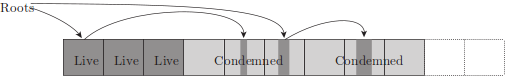
\includegraphics{figures/conc_2a}
    \caption
      {Αρχική διαμόρφωση αλγορίθμου Compressor. Όλες οι
       σελίδες ανήκουν στο χώρο-από.}
  \end{subfigure}

  \begin{subfigure}[b]{1.0\textwidth}
    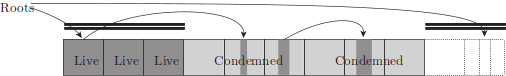
\includegraphics{figures/conc_2b}
    \caption
      {Υπολογισμός πληροφοριών προώθησης και προστασία όλων
       των σελίδων του χώρου-προς. Μεταξύ αυτών είναι οι
       δεσμευμένες σελίδες προς τις οποίες θα μεταφερθούν
       ζωντανά αντικείμενα και οι ζωντανές σελίδες που δεν
       έχουν καταδικασθεί για εκκένωση. Στη συνέχεια οι ρίζες
       των τροποποιητών δείχνουν προς το χώρο-προς. Τα νήματα
       τροποποιητές που θα προσπαθήσουν να προσπελάσουν μια
       προστατευμένη σελίδα του χώρου-προς θα παγιδευθούν.}
  \end{subfigure}
  
  \begin{subfigure}[b]{1.0\textwidth}
    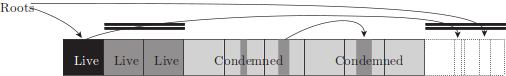
\includegraphics{figures/conc_2c}
    \caption
      {Η παγίδευση σε μία ζωντανή σελίδα προωθεί τους δείκτες
       που περιλαμβάνονται σε αυτή ώστε να αναφέρονται προς
       τα αντίγραφα στο χώρο-προς των προορισμών τους. Η προστασία
       της ζωντανής σελίδας αίρεται όταν έχουν πλέον προωθηθεί
       όλοι οι δείκτες αυτής.}
  \end{subfigure}
  
  \begin{subfigure}[b]{1.0\textwidth}
    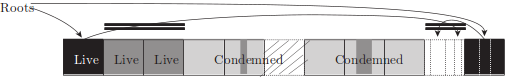
\includegraphics{figures/conc_2d}
    \caption
      {Η παγίδευση σε μία δεσμευμένη σελίδα του χώρου-προς
       γεμίζει τη σελίδα εκκενώνοντας σελίδες του χώρου-από.
       Τα πεδία δείκτες των αντικειμένων αυτών ενημερώνονται
       ώστε να δείχνουν προς το χώρο-προς. Στη συνέχεια αίρεται
       η προστασία της σελίδας του χώρου-προς και καταργείται
       η απεικόνιση προς πλήρως εκκενωμένες σελίδες του
       χώρου-από.}
  \end{subfigure}
  
  \begin{subfigure}[b]{1.0\textwidth}
    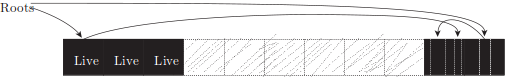
\includegraphics{figures/conc_2e}
    \caption
      {Η συμπύκνωση ολοκληρώνεται όταν όλες οι ζωντανές
       σελίδες έχουν σαρωθεί, όλοι οι δείκτες που αυτές
       περιλαμβάνουν έχουν προωθηθεί, όλα τα ζωντανά
       αντικείμενα καταδικασμένων σελίδων έχουν αντιγραφεί
       στο χώρο-προς και όλες οι αναφορές των τελευταίων
       έχουν προωθηθεί.}
  \end{subfigure}    
  \caption
    [Ταυτόχρονη εκτέλεση αλγορίθμου Compressor]
    {Ταυτόχρονη εκτέλεση αλγορίθμου Compressor.}
  \label{fig:conc_2}
\end{figure}

\section{Ταυτόχρονη Καταμέτρηση Αναφορών}
Εξετάσαμε τη συλλογή με καταμέτρηση αναφορών στο κεφάλαιο
~\ref{ch:refcnt}. Είδαμε πώς τα βασικά μειονεκτήματα της
απλοϊκής καταμέτρησης αναφορών αφορούν στην αδυναμία συλλογής
κύκλων σκουπιδιών και το υψηλό κόστος της διαχείρισης των
μετρητών αναφορών, ειδικά σε καταστάσεις συναγωνισμού μεταξύ
πολλαπλών νημάτων τροποποιητών. Ο αλγόριθμος Recycler (αλγόριθμος~\ref{alg:refcnt_5})
χρησιμοποιώντας την τεχνική της
δοκιμαστικής διαγραφής λύνει το πρόβλημα της αδυναμίας συλλογής
κύκλων σκουπιδιών. Η καταμέτρηση αναφορών με αναβολή αποτρέπει
τα νήματα τροποποιητές από το να μεταβάλλουν τους μετρητές
αναφορών τοπικών μεταβλητών, ενώ τέλος η καταμέτρηση αναφορών
με συγκέντρωση αποφεύγει τις περιττές ενημερώσεις των μετρητών
αναφοράς που ακυρώνονται από αργότερες λειτουργίες εγγραφής
δεικτών από τα νήματα τροποποιητές. Και οι τρεις λύσεις απαιτούν
την διακοπή του κόσμου την ώρα που ο συλλέκτης ενημερώνει τους
μετρητές αναφοράς και ανακτά τη μνήμη από αντικείμενα σκουπίδια. 
Εξετάζουμε τώρα πώς η απαίτηση για διακοπή του κόσμου μπορεί
να αποφευχθεί καθώς και ποιες αλλαγές απαιτούνται ώστε ένας
συλλέκτης με καταμέτρηση αναφορών να εκτελεστεί ταυτόχρονα με
τα νήματα τροποποιητές.

\subsection{Απλοϊκή καταμέτρηση αναφορών}
Η ορθότητα ενός συλλέκτη σκουπιδιών με καταμέτρηση αναφορών
απαιτεί την εξασφάλιση της ισχύος της αναλλοίωτης ότι ο μετρητής
αναφοράς κάθε αντικειμένου ισούται με το πλήθος των αναφορών
προς αυτό. Η εξασφάλιση της αναλλοίωτης είναι ιδιαίτερα περίπλοκη
όταν εμπλέκονται πολλαπλά νήματα τροποποιητές. Εκ πρώτης όψεως,
φαίνεται πώς η ασφαλής εκτέλεση της λειτουργίας \textenglish{\textproc{Write}}
είναι πιο δύσκολη από την ασφαλή εκτέλεση της λειτουργίας
\textenglish{\textproc{Write}}. Η ενημέρωση ενός δείκτη περιλαμβάνει τρεις
ενέργειες: την αύξηση του μετρητή αναφορών του νέου αντικειμένου
αναφοράς, τη μείωση του μετρητή αναφορών του παλαιού αντικειμένου
αναφοράς και την εγγραφή του δείκτη. Ο συντονισμός των ενεργειών
αυτών είναι απαραίτητος ούτως ώστε να αποφεύγεται η πρόωρη
αποδέσμευση αντικειμένων (λόγω για παράδειγμα προσωρινής μηδενικής
τιμής μετρητών αναφοράς) όσο και η επ' άπειρον αιώρηση σκουπιδιών
στο σωρό.

Η δυσκολία της ταυτόχρονης συλλογής σκουπιδιών με καταμέτρηση αναφορών δεν έγκειται μόνο στην
εξασφάλιση της ατομικής αύξησης και μείωσης μετρητών αναφορών. Το δυσκολότερο πρόβλημα αφορά
το συγχρονισμό των τροποποιήσεων των μετρητών αναφοράς με τις φορτώσεις και αποθηκεύσεις
δεικτών. Ένας τρόπος επίτευξης της ατομικότητας των λειτουργιών \textenglish{\textproc{Read}} και 
\textenglish{\textproc{Write}} του τροποποιητή είναι το κλείδωμα του αντικειμένου στο οποίο ανήκει το πεδίο
που διαβάζεται η γράφεται. 

Είναι επιθυμητή η εύρεση μιας λύσης που δε χρησιμοποιεί κλειδώματα αλλά πρωταρχικές εντολές
των οποίων η ατομικότητα εξασφαλίζεται από το υλικό. Δυστυχώς, οι πρωταρχικές 
εντολές που αφορούν μόνο μία θέση μνήμης δεν επαρκούν για την εξασφάλιση της ασφάλειας.
Ο Detlefs κ.ά. \cite{DBLP:conf/podc/DetlefsMMS01} [2001,2002b] δείχνουν πώς η λειτουργία \textenglish{\textproc{CompareAndSwap2}}, η οποία
ατομικά ενημερώνει δύο διαφορετικές θέσεις μνήμης επαρκεί. Παρότι δεν είναι αρκετή για τη διατήρηση
ακριβών τιμών των μετρητών αναφορών για κάθε χρονική στιγμή, η χρήση της εξασφαλίζει την ασθενέστερη
αναλλοίωτη πώς:
\begin{itemize}
\item όσο υπάρχει τουλάχιστον μια αναφορά προς ένα αντικείμενο, ο μετρητής αναφορών αυτού θα είναι
μη μηδενικός και
\item αν δεν υπάρχουν αναφορές προς ένα αντικείμενο, ο μετρητής αναφορών του τελικώς θα μηδενισθεί.
\end{itemize}

\subsection{Καταμέτρηση αναφορών με χρήση απομονωτή}
Οι αλγόριθμοι συλλογής σκουπιδιών με πρόθυμη καταμέτρηση
αναφορών απαιτούν τη χρήση είτε κλειδωμάτων είτε πρωταρχικών
ατομικών εντολών που τροποποιούν πολλές λέξεις μνήμης
ταυτόχρονα. Οι μηχανισμοί κλειδωμάτων δεν είναι ιδιαίτερα
φθηνοί, ενώ οι ατομικές πρωταρχικές εντολές πολλαπλών θέσεων
μνήμης δεν προσφέρονται από όλες τις αρχιτεκτονικές συνόλου
εντολών. Η καταμέτρηση αναφορών με αναβολή περιορίζει κάπως
το πρόβλημα με τη μη εφαρμογή λειτουργιών καταμέτρησης αναφορών
σε τοπικές μεταβλητές και την αναβολή της ανάκτησης μνήμης
αντικειμένων με μηδενικό μετρητή αναφορών. H
\textbf{καταμέτρηση αναφορών με χρήση απομονωτή} υποστηρίζει
την εκτέλεση πολυνηματικών εφαρμογών χρησιμοποιώντας απλές
εντολές φόρτωσης και αποθήκευσης στο φράγμα εγγραφής του
τροποποιητή.

Ο DeTreville \cite{detreville1990experience} σε έναν υβριδικό
συλλέκτη για τη γλώσσα Modula-2+ που χρησιμοποιεί έναν
εφεδρικό συλλέκτη με σήμανση και εκκαθάριση για την
αντιμετώπιση κύκλων σκουπιδιών, προκειμένου να αποφύγει το
κόστος του συγχρονισμού των λειτουργιών καταμέτρησης αναφορών
από διαφορετικά νήματα τροποποιητές, ανέθετε στα τελευταία
να καταχωρούν τις διευθύνσεις του παλαιού και του νέου
αντικειμένου αναφοράς ενός δείκτη σε έναν απομονωτή. Στη
συνέχεια, ένα ξεχωριστό νήμα καταμέτρησης αναφορών επεξεργάζεται
το χώρο καταχώρισης και προσαρμόζει τους μετρητές αναφορών
εξασφαλίζοντας με τον τρόπο αυτό την ατομικότητα των ενημερώσεων.
Δυστυχώς όμως η καταμέτρηση αναφορών με χρήση απομονωτή δεν
εξαφανίζει το πρόβλημα του συντονισμού των λειτουργιών
καταμέτρησης αναφορών και της εγγραφής του δείκτη. Ο
DeTreville πρότεινε δύο λύσεις, από τις οποίες όμως καμία δεν
είναι εξ ολοκλήρου ικανοποιητική. Η πρώτη του προσέγγιση αφορά
στην προστασία με κλείδωμα ολόκληρης της λειτουργίας
\textenglish{\textproc{Write}}. Για να αποφύγει το κόστος της ατομικής
εκτέλεσης κάθε λειτουργίας \textenglish{\textproc{Write}}, η δεύτερη λύση
του παρέχει σε κάθε νήμα τροποποιητή το δικό του τοπικό
απομονωτή, ο οποίος περιοδικά περνά στον έλεγχο του νήματος
καταμέτρησης αναφορών. Η προσέγγιση αυτή ωστόσο μεταφέρει
την ευθύνη της εξασφάλισης της ατομικής εκτέλεσης των
λειτουργιών \textenglish{\textproc{Write}} στον προγραμματιστή, ο οποίος
επιβαρύνεται με το ιδιαίτερα επίπονο έργο του χειρισμού
κλειδωμάτων.

Οι Bacon και Rajan \cite{DBLP:conf/ecoop/BaconR01} επίσης
παρέχουν σε κάθε νήμα τροποποιητή το δικό του τοπικό
απομονωτή, απαιτούν όμως η ενημέρωση ενός δείκτη να είναι
ατομική. Το φράγμα εγγραφής του τροποποιητή σε έναν επεξεργαστή
προσθέτει την παλαιά και την καινούρια τιμή του πεδίου $i$ ενός
αντικειμένου στον τοπικό απομονωτή $localUpdates$. Η καταμέτρηση
αναφορών των τοπικών μεταβλητών αναβάλλεται και πάλι, ενώ για
να αποτραπεί η πρόωρη διαγραφή αντικειμένων, ο χρόνος διαιρείται
σε \textbf{εποχές} χρησιμοποιώντας έναν καθολικό αριθμό εποχής
και τοπικούς αριθμούς εποχής για κάθε νήμα τροποποιητή.
Περιοδικά, όπως και στην καταμέτρηση αναφορών με αναβολή,
ένας επεξεργαστής θα διακόψει την εκτέλεση ενός νήματος
τροποποιητή και θα εξετάσει όλες τις τοπικές στοίβες,
καταχωρώντας τις αναφορές που βρίσκει σε έναν τοπικό απομονωτή
$myStackBuffer$. Στη συνέχεια ο επεξεργαστής μεταφέρει τους
απομονωτές $myStackBuffer$ και $myUpdates$ στο συλλέκτη και
ενημερώνει τον τοπικό αριθμό εποχής $e$. Τέλος, δρομολογεί
το νήμα συλλέκτη στον επόμενο επεξεργαστή πριν επαναφέρει
σε λειτουργία το σταματημένο νήμα τροποποιητή.

Το νήμα συλλέκτης εκτελείται στον επόμενο επεξεργαστή. Σε
κάθε κύκλο συλλογής $k$, ο συλλέκτης εφαρμόζει τις αυξήσεις
μετρητών αναφοράς της εποχής $k$ και τις μειώσεις μετρητών
αναφοράς της εποχής $k-1$. Τέλος, ενημερώνει τον καθολικό
αριθμό εποχής. Το πλεονέκτημα της μεθόδου είναι πώς ποτέ
δεν απαιτείται η αναστολή λειτουργίας όλων των νημάτων
τροποποιητών: ο συλλέκτης λειτουργεί εν-τη-πτήσει.

\begin{algorithm}
  \caption{Ταυτόχρονη καταμέτρηση αναφορών με χρήση απομονωτή}
  \label{alg:conc_4}
  \begin{algorithmic}[1]
    \State \textbf{shared} $epoch$
    \State \textbf{shared} $updatesBuffer[]$ \Comment{one buffer per epoch}
    \Statex
    \Procedure{Write}{$src$, $i$, $ref$}
      \If{$src=Roots$}
        \State $src[i] \gets ref$
      \Else
        \State $old \gets$ \Call{AtomicExchange}{$\&src[i]$, $ref$}
        \State \Call{log}{$old$, $ref$}
      \EndIf
    \EndProcedure
    \Statex
    \Procedure{log}{$old$, $new$}
      \State $myUpdates \gets myUpdates + [<old, new>]$
    \EndProcedure
    \Statex
    \Procedure{collect}{\null}
      \State $myStackBuffer \gets []$
      \ForAll{\textbf{local} $ref \; \textbf{in} \; myStacks$} \Comment{deferred reference counting}
        \State $myStackBuffer \gets myStackBuffer + [<ref, ref>]$
        \State \textbf{atomic}
        \State $updatesBuffer[e] \gets updatesBuffer[e] + myStackBuffer$
        \State \textbf{atomic}
        \State $updatesBuffer[e] \gets updatesBuffer[e] + myUpdates$
      \EndFor
        \State $myUpdates \gets []$
        \State $e \gets e + 1$
        \Statex
        \State $me \gets myProcessorId$
        \If{$me < MAX\_PROCESSORS$}
          \State \Call{schedule}{$collect$, $me+1$} \Comment{schedule collect() on the next processor}
        \Else \Comment{the last processor updates the reference counts}
          \ForAll{$<old, new> \; \textbf{in} \; updatesBuffer[epoch]$}
            \State \Call{addReference}{$old$}
          \EndFor
          \ForAll{$<old, new> \; \textbf{in} \; updatesBuffer[epoch]$}
            \State \Call{addReference}{$old$}
          \EndFor
          \State \Call{release}{$updatesBuffer[epoch-1]$} \Comment{free the old buffer}
          \State $epoch \gets epoch+1$
        \EndIf
    \EndProcedure
  \end{algorithmic}
\end{algorithm}

\subsection{Ταυτόχρονη κυκλική καταμέτρηση αναφορών}
Ο αλγόριθμος Recycler
\cite{DBLP:conf/pldi/BaconALRS01, DBLP:conf/ecoop/BaconR01}
ανακτά τη μνήμη από κύκλους σκουπιδιών εξερευνώντας υποψήφιους
υπογράφους και εφαρμόζοντας δοκιμαστική διαγραφή στους μετρητές
αναφορών. Παρότι η χρήση απομονωτή επιτυχώς μεταβιβάζει την
καταμέτρηση αναφορών σε έναν εφεδρικό επεξεργαστή, ο αλγόριθμος
Recycler αντιμετωπίζει τρία προβλήματα στην προσπάθεια συλλογής
κύκλων σκουπιδιών σε ένα περιβάλλον ταυτοχρονισμού:

\begin{enumerate}
\item Δεν μπορεί να εγγυηθεί πώς θα εξερευνήσει εκ νέου τον
  ίδιο υπογράφο καθώς ο γράφος μπορεί να έχει τροποποιηθεί
  από τα νήματα τροποποιητές ενόσω αυτός εντοπίζει κύκλους
  σκουπιδιών.
\item Διαγραφές δεικτών ενδέχεται να αποσυνδέσουν το γράφο.
\item Οι μετρητές αναφορών μπορεί να είναι ανενημέρωτοι.
\end{enumerate}

Η ασύγχρονη έκδοση του αλγορίθμου λειτουργεί σε δύο φάσεις
για να επιλύσει τα παραπάνω προβλήματα. Η πρώτη φάση είναι
λίγο πολύ η σύγχρονη εκδοχή του αλγορίθμου που παρουσιάσθηκε
στο κεφάλαιο \ref{ch:refcnt}. Ωστόσο ο ασύγχρονος Recycler
αναβάλλει την αποδέσμευση της μνήμης αντικειμένων που
εντοπίζει η διαδικασία \textenglish{\textproc{collectWhite}} (βλέπε
\ref{alg:refcnt_5}) μέχρι την επόμενη φάση, η οποία ελέγχει
ότι αυτά είναι ακόμη σκουπίδια. Η προσέγγιση αυτή παρουσιάζει
τα ακόλουθα μειονεκτήματα. Θεωρητικά και σπάνια στην πράξη
είναι πιθανόν ορισμένοι κύκλοι σκουπιδιών να μη συλλεγούν:
δεν υπάρχει εγγύηση πληρότητας του ασύγχρονου συλλέκτη.
Επιπλέον, η δοκιμαστική διαγραφή δε μπορεί να χρησιμοποιήσει
τον αυθεντικό μετρητή αναφορών αλλά έναν ειδικό κυκλικό
μετρητή αναφορών που επίσης αποθηκεύεται στην επικεφαλίδα
των αντικειμένων. Τρίτον, ο αλγόριθμος πρέπει να εξερευνήσει
εκ νέου τους υποψήφιους κύκλους σκουπιδιών στη δεύτερη φάση,
για να αποφύγει τη λανθασμένη αποδέσμευση ανακύκλωση ζωντανών
αντικειμένων.

Το βασικό πρόβλημα είναι πώς ο συλλέκτης Recycler προσπαθεί
να εφαρμόσει έναν αλγόριθμο που έχει σχεδιασθεί για σύγχρονη
συλλογή σε έναν ταυτόχρονο κόσμο όπου η τοπολογία του γράφου
αντικειμένων διαρκώς μεταβάλλεται.

\begin{figure}
  \centering
  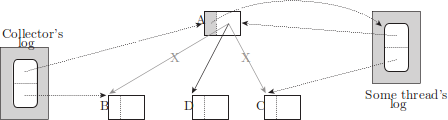
\includegraphics{figures/conc_4}
  \caption
    [Ταυτόχρονη καταμέτρηση αναφορών με συγκέντρωση.]
    {Ταυτόχρονη καταμέτρηση αναφορών με συγκέντρωση. Στη
     διάρκεια της προηγούμενης εποχής το αντικείμενο $A$
     τροποποιήθηκε ώστε να δείχνει στο αντικείμενο $C$
     και οι τιμές των πεδίων του αποθηκεύθηκαν σε κάποιον
     τοπικό απομονωτή καταγραφής. Ωστόσο, το αντικείμενο
     $A$ έχει τροποποιηθεί ξανά σε αυτήν την εποχή (δείχνει
     πλέον στο αντικείμενο $D$) και συνεπώς έχει σημανθεί
     ως βρώμικο και καταγραφεί ξανά. Το αρχικό αντικείμενο
     αναφοράς $B$ μπορεί να βρεθεί στον καθολικό χώρο
     καταγραφής, όπως και στο σχήμα~\ref{fig:refcnt_2}. Η
     αναφορά προς το αντικείμενο $C$ μπορεί να βρεθεί στον
     τοπικό απομονωτή καταγραφής ενός νήματος τροποποιητή,
     προς τον οποίο υπάρχει δείκτης από το αντικείμενο
     $A$.} 
\end{figure}

\subsection{Λήψη ενός στιγμιοτύπου του σωρού}
Στο κεφάλαιο~\ref{ch:refcnt} είδαμε πώς η καταμέτρηση
αναφορών με συγκέντρωση παρέχει στο συλλέκτη ένα στιγμιότυπο
του σωρού. Σε έναν τοπικό σε κάθε νήμα τροποποιητή απομονωτή,
ο οποίος μεταφέρεται σύγχρονα στο συλλέκτη, αποθηκεύονται
αντίγραφα αντικειμένων των οποίων πεδία δείκτες έχουν
τροποποιηθεί. Η λειτουργία όλων των νημάτων τροποποιητών
αναστέλλεται στην αρχή ενός κύκλου συλλογής, οι απομονωτές
διαβιβάζονται στο συλλέκτη και δεσμεύεται μνήμη για νέους
απομονωτές. Ο συλλέκτης απλώς χρησιμοποιεί το αντίγραφο ενός
αντικειμένου για να βρει τα παλαιά αντικείμενα αναφοράς των
δεικτών αυτού και να μειώσει τους μετρητές αναφορών αυτών,
ενώ χρησιμοποιεί την τρέχουσα κατάσταση του αντικειμένου για
να αυξήσει τους μετρητές αναφορών των νέων αντικειμένων
αναφορών των δεικτών αυτού. 

Το νήμα καταμέτρησης αναφορών μπορεί να εκτελείται ταυτόχρονα
με τα νήματα τροποποιητές. Στην περίπτωση αυτή, η εκτέλεση
των νημάτων τροποποιητών αναστέλλεται προσωρινά, μέχρις ότου
οι απομονωτές αυτών μεταβιβασθούν στο συλλέκτη. Μόλις
ολοκληρωθεί η μεταφορά, επανεκκινείται η εκτέλεση των νημάτων
τροποποιητών. Ο συλλέκτης είναι επιφορτισμένος με τη διόρθωση
των μετρητών αναφοράς των παλαιών και των νέων παιδιών κάθε
τροποποιημένου αντικειμένου. Η μείωση των μετρητών αναφοράς των
παλαιών παιδιών γίνεται εύκολα, όπως και πριν χρησιμοποιώντας
το αντίγραφο ενός αντικειμένου. Η αύξηση όμως των μετρητών
αναφοράς των παιδιών ενός αντικειμένου τη στιγμή μεταφοράς των
απομονωτών είναι πιο περίπλοκη, καθώς το αντικείμενο ενδέχεται
να έχει τροποποιηθεί εκ νέου.

Αν το αντικείμενο παραμένει καθαρό, τότε η κατάσταση του δεν
έχει αλλάξει και οι μετρητές αναφορών των τρεχόντων παιδιών
του αυξάνονται. Αν πάλι το αντικείμενο έχει τροποποιηθεί από
τη στιγμή μεταφοράς των απομονωτών, τότε έχει ξανασημανθεί ως
βρώμικο και η κατάσταση του τη στιγμή της μεταφοράς μπορεί να
βρεθεί σε ένα φρέσκο (καινούριο) απομονωτή κάποιου νήματος
τροποποιητή. Ο βρώμικος δείκτης του αντικειμένου αναφέρεται
σε αυτόν τον απομονωτή καταχώρισης, ο οποίος μπορεί να
αναγνωσθεί χωρίς να απαιτείται ο συγχρονισμός του συλλέκτη
με το νήμα στο οποίο ο τελευταίος ανήκει.

\subsection{Καταμέτρηση αναφορών με ολισθαίνουσες όψεις}
Για τη λήψη ενός στιγμιοτύπου του σωρού, αναστέλλεται η
εκτέλεση όλων των νημάτων τροποποιητών ταυτόχρονα προκειμένου
να πραγματοποιηθεί η μεταφορά των απομονωτών. Η τεχνική των
\textbf{ολισθαινουσών όψεων} χαλαρώνει τον παραπάνω περιορισμό
και προσφέρει τη δυνατότητα να διακόπτεται η εκτέλεση ενός
μόνο νήματος κάθε φορά. Είναι προφανές πώς αυτή η προσέγγιση
έχει ως αποτέλεσμα να παρέχεται στο συλλέκτη μια παραμορφωμένη
εικόνα του σωρού. Οι τιμές διαφορετικών αντικειμένων
καταγράφονται και μεταβιβάζονται στο νήμα συλλέκτη σε
διαφορετικές χρονικές στιγμές. Η τεχνική δεν απαιτεί τη χρήση
κλειδωμάτων ούτε και ατομικών πρωταρχικών λειτουργιών υλικού,
αλλά συντονίζει κάθε νήμα τροποποιητή με το νήμα συλλέκτη με
τη χρήση 4 χειραψιών όμοιων με εκείνες που χρησιμοποιούν οι
Doligez και Gonthier \cite{DBLP:conf/popl/DoligezG94}. Η
τεχνική των ολισθαινουσών όψεων χρησιμοποιείται ευρέως για
απλή, καθαρή καταμέτρηση αναφορών από τους Levanoni και
Petrank \cite{levanoni1999scalable, DBLP:conf/oopsla/LevanoniP01,
DBLP:journals/toplas/LevanoniP06}, για τη διαχείριση της
παλαιάς γενεάς γενεαλογικών συλλεκτών από τους Azatchi και
Petrank, \cite{DBLP:conf/oopsla/AzatchiLPP03}) καθώς και
σε συνδυασμό με κυκλική καταμέτρηση αναφορών από τον Paz
κ.ά. \cite{DBLP:conf/cc/PazPBKR05, DBLP:conf/cc/PazP07}.

\section{Θέματα προς εξέταση}
\subsection{Ταυτόχρονη σήμανση και εκκαθάριση}
Πολλά από τα ζητήματα που αφορούν την ταυτόχρονη συλλογή
σκουπιδιών με σήμανση και εκκαθάριση είναι κοινά για τους
περισσότερους ταυτόχρονους συλλέκτες. Η σχεδίαση ενός
ταυτόχρονου συλλέκτη είναι σαφώς πιο πολύπλοκη από τη
σχεδίαση ενός συλλέκτη που λειτουργεί με παύση του κόσμου.
Προκύπτει το ερώτημα κατά πόσον οι απαιτήσεις από το συλλέκτη
δικαιολογούν αυτήν την επιπλέον πολυπλοκότητα, καθώς μια
απλούστερη λύση, όπως η χρήση ενός γενεαλογικού συλλέκτη
να είναι αρκετή.

Οι γενεαλογικοί συλλέκτες σκουπιδιών προσφέρουν αναμενόμενους
χρόνους παύσης της τάξης των χιλιοστών του δευτερολέπτου για
τις περισσότερες εφαρμογές. Ωστόσο στη χειρότερη περίπτωση,
όπου και πρέπει να συλλεγεί ολόκληρος ο σωρός ο χρόνος παύσης
μιας εφαρμογής μπορεί να αυξηθεί υπερβολικά ανάλογα με το
μέγεθος του σωρού, τον όγκο των ζωντανών αντικειμένων κ.ο.κ.
Οι ταυτόχρονοι συλλέκτες από την άλλη πλευρά προσφέρουν
συντομότερους και πιο προβλέψιμους χρόνους παύσης.

Η ταυτόχρονη συλλογή με σήμανση και εκκαθάριση μπορεί όπως
και η μη ταυτόχρονη συλλογή με σήμανση και εκκαθάριση να
οδηγήσει σε κατακερματισμό του σωρού. Η συλλογή με αντιγραφή
και η συλλογή με σήμανση και συμπύκνωση εκτός από το ότι
αντιμετωπίζουν τον κατακερματισμό της μνήμης επιτρέπουν
επίσης την σειριακή εκχώρηση μνήμης, η οποία μπορεί να
είναι ταχύτερη από την εκχώρηση με χρήση ελεύθερης λίστας
και μπορεί επίσης να παρέχει καλύτερη τοπικότητα αναφορών
στα νήματα τροποποιητές. Από την άλλη πλευρά βέβαια οι συλλέκτες
σήμανσης και εκκαθάρισης χρησιμοποιούν αποδοτικότερα το
διαθέσιμο χώρο μνήμης σε σύγκριση με τους συλλέκτες αντιγραφής
καθώς δεν απαιτούν την ύπαρξη ενός εφεδρικού χώρου αντιγραφής.
Επιπλέον, οι μη μετακινούντες ταυτόχρονοι συλλέκτες έχουν
το εξής πλεονέκτημα σε σχέση με τους μετακινούντες ταυτόχρονους
συλλέκτες: η εξασφάλιση της συνέπειας του σωρού είναι σχετικά
απλή. Όλοι οι ταυτόχρονοι συλλέκτες απαιτούν από τα νήματα
τροποποιητές να τους ενημερώνουν σχετικά με τη μεταβολή της
τοπολογίας του σωρού ούτως ώστε να αποτραπεί η περίπτωση κάποιο
νήμα τροποποιητής να κρύβει αντικείμενα από το συλλέκτη. Ωστόσο,
οι ταυτόχρονοι μετακινούντες συλλέκτες πρέπει επιπλέον να
εξασφαλίσουν τόσο πώς μόνο ένα νήμα συλλέκτης μετακινεί ένα
αντικείμενο όσο και πώς η ενημέρωση όλων των δεικτών προς
ένα μετακινηθέν αντικείμενο εμφανίζεται να πραγματοποιείται
ατομικά στα νήματα τροποποιητές.

Τέλος η ταυτόχρονη συλλογή με σήμανση και εκκαθάριση προσφέρει
έναν αριθμό από σχεδιαστικές επιλογές υλοποίησης. Τα καινούρια
αντικείμενα μπορούν να εκχωρούνται είτε ως μαύρα, γκρι ή λευκά.
Ένα νέο αντικείμενο εκχωρείται πάντοτε ως μαύρο σε ένα μαύρο
τροποποιητή, ενώ ένας γκρι τροποποιητής προσφέρει περισσότερες
επιλογές. Τα νέα αντικείμενα μπορούν να εκχωρούνται ως μαύρα,
γκρι, ή λευκά και επιπλέον η απόφαση μπορεί να διαφέρει ανάλογα
με τη φάση του κύκλου συλλογής, τις αρχικές τιμές των πεδίων
του καινούριου αντικειμένου ή την πρόοδο της φάσης της εκκαθάρισης.

\subsection{Ταυτόχρονη αντιγραφή και συμπύκνωση}
Η ταυτόχρονη συλλογή αντιγραφής και σήμανσης και συμπύκνωσης
μειώνει τον κατακερματισμό της μνήμης και επίσης αποτρέπει
την εμφάνιση μεγάλων χρόνων παύσης. Όπως και στις άλλες
τεχνικές ταυτόχρονης συλλογής σκουπιδιών, ο συλλέκτης πρέπει να προστατεύεται
από τις ενέργειες του τροποποιητή ώστε να μην υπάρχουν
μη ορατά στο συλλέκτη προσβάσιμα αντικείμενα. Όμως επειδή
ο συλλέκτης μετακινεί αντικείμενα πρέπει και ο τροποποιητής
να προστατευθεί από τις ενέργειες του συλλέκτη ώστε να μην
προσπελάσει μη έγκυρα αντίγραφα αντικειμένων. Ο Baker
\cite{DBLP:journals/cacm/Baker78} προστατεύει τον τροποποιητή
εξασφαλίζοντας την διατήρηση μιας αναλλοίωτης του χώρου-προς
η οποία δεν επιτρέπει στον τροποποιητή τη διατήρηση δεικτών
προς αντικείμενα του χώρου-από. Ο Brooks \cite{DBLP:conf/lfp/Brooks84}
προστατεύει τον τροποποιητή επιτρέποντας του να συνεχίζει
να λειτουργεί στο χώρο-από και αναθέτοντάς του την ενημέρωση
των διευθύνσεων προώθησης προς αντικείμενα του χώρου-προς
καθώς αυτά δημιουργούνται. 
Η συμπύκνωση μπορεί να πραγματοποιηθεί με παρόμοιους τρόπους
χωρίς την απαίτηση να αντιγράφονται όλα τα αντικείμενα σε
έναν κύκλο συλλογής.

Η εφαρμογή μιας εκ των των παραπάνω τεχνικών πάντως μπορεί να
έχει ως αποτέλεσμα μεγαλύτερους χρόνους παύσης σε σύγκριση
με μη μετακινούντες ταυτόχρονους συλλέκτες: σε οποιαδήποτε
προσπάθεια προσπέλασης του σωρού ο τροποποιητής μπορεί να
παγιδευθεί και χρειασθεί να περιμένει μέχρις ότου ένα ή
περισσότερα αντικείμενα μετακινηθούν.

\subsection{Ταυτόχρονη καταμέτρηση αναφορών}
Το βασικό πρόβλημα της καταμέτρησης αναφορών σχετίζεται με το
πώς θα εξασφαλισθεί πώς οι μετρητές αναφορών των αντικειμένων
έχουν σωστές τιμές ενώ ο γράφος αντικειμένων τροποποιείται
ταυτόχρονα. Η απλούστερη λύση είναι να απαιτείται από τα νήματα
τροποποιητές να κλειδώνουν ένα αντικείμενο πριν το τροποποιήσουν.
Συνήθως όμως το κόστος των κλειδωμάτων θεωρείται υψηλό και συνεπώς
πρέπει να βρεθούν εναλλακτικές προσεγγίσεις. Οι τρέχουσες λύσεις
βασίζονται στην αποφυγή των καταστάσεων συναγωνισμού μεταξύ
νημάτων τροποποιητών που μπορεί να διακινδυνεύσουν την συνέπεια
των μετρητών αναφορών. Ο διαχειριστής μνήμης ενδιαφέρεται μόνο
να εξασφαλίσει τη συνέπεια του σωρού: δεν είναι δική του ευθύνη
η εξασφάλιση της ορθότητας του προγράμματος χρήστη.

Για να διατηρηθεί η συνοχή του σωρού, απαιτείται η σειριοποίηση
των εγγραφών δεικτών και των λειτουργιών ενημέρωσης των μετρητών
αναφορών. Μια μερική λύση είναι η χρήση της καταμέτρησης αναφορών
με αναβολή, καθώς έτσι αναβάλλεται η αποδέσμευση της μνήμης των 
σκουπιδιών η οποία μάλιστα ανατίθεται σε ένα ξεχωριστό νήμα
συλλέκτη. Ωστόσο η λύση αυτή αφορά μόνο τις φορτώσεις και
αποθηκεύσεις δεικτών και όχι τις εγγραφές σε πεδία δείκτες στο
εσωτερικό αντικειμένων. Προκύπτει έτσι το ερώτημα του πώς μπορούν
οι ενημερώσεις μετρητών αναφοράς που απορρέουν από τις εγγραφές
πεδίων δεικτών να ανατεθούν από τα νήματα τροποποιητές σε ένα
νήμα συλλέκτη. Η απλούστερη λύση είναι κάθε νήμα τροποποιητής
να απομονώνει τις λειτουργίες καταμέτρησης αναφορών του και να
τις περνά περιοδικά στο νήμα συλλέκτη. Η καταμέτρηση αναφορών
με συγκέντρωση πηγαίνει την παραπάνω ιδέα ένα βήμα πιο πέρα:
λαμβάνοντας ένα στιγμιότυπο των αντικειμένων πριν αυτά τροποποιηθούν
επιτρέπει στο νήμα συλλέκτη να αποφύγει την εφαρμογή περιττών
ενημερώσεων των μετρητών αναφορών. Και στις δύο περιπτώσεις
πάντως η διαχείριση των μετρητών αναφορών και η αποδέσμευση
αντικειμένων διαχωρίζεται πλήρως από τις εγγραφές δεικτών
και πραγματοποιείται εξ' ολοκλήρου από ένα ξεχωριστό νήμα
συλλέκτη ή και πολλαπλά νήματα συλλέκτες που τρέχουν παράλληλα.
Η λήψη ενός στιγμιοτύπου της κατάστασης του σωρού επίσης
απλοποιεί την κυκλική καταμέτρηση αναφορών. Οι αλγόριθμοι
δοκιμαστικής διαγραφής πρέπει να διασχίσουν έναν υπογράφο του
σωρού πολλές φορές. Διασχίζοντας το στιγμιότυπο, ο συλλέκτης
μπορεί να εξασφαλίσει πώς εξερευνά τον ίδιο υπογράφο κάθε
φορά παρά τις ταυτόχρονες δραστηριότητες νημάτων τροποποιητών.

\end{greek}
